%%%%%%%%%%%%%%%%%%%%%%%%%%%%%%%%%%%%%%%%%%%%%%%%%%%%%%%%%%%%%%%%%%%%%%%%%%%%%%%%%%%
%%Anna University sample latex thesis format for UG thesis
%--------------------------------
%%This is the main file that includes the front matter and other chapter links. 
%%Chapters are placed within the folder named 1, 2,...  
%%To compile, run the command `pdflatex authesis.tex' in the terminal. 
%%Some packages may not be needed. Comment the ones, that are not needed. 
%%Images can be saved in the format of *.png. 
%%------------------------------------------------------
%% Authors:
%%Originally used by Dr. Mary Anita Rajam and then modified by Dr. Bama Srinivasan according to the latest Anna University regulations. %%Please report changes to bama@annauniv.edu, chorse@gmail.com %%
%%Acknowledgement: Thanks to Dr.Ranjani Parthasarathi, who relentlessly and patiently guided Bama Srinivasan.
%---------------------------------------------------------
%% Modification added:
%%new file apalikem is added, which gives a neat reference list with 1, 2...
%%aureportm has appendix starting with Arabic numbers
%% Disclaimer: Check with the latest Anna University regulations before working with this format.
%% Changes as on July 2016 
%% 1. Changed the appendix back to alpha mode in aureport.cls
%% 2. Table of contents - reduced the top margin and spacing
%% 3. Added the counter depth for sections to 4 in aureport.cls
%% 4. Deleted chapter number, title and page number in TOC
%% 5. Reduced the top space in chapter titles from 6.5 cms to 5.5 cms in aureport.cls
%% 6. Changes in references use the package natbib and style unsrt. Include a .bib file for the bibliography
%$$$$$$$$$$$$$$$$$$$$$$$$$$$$$$$$$$$$$$$$$$$$$$$$$$$$$$$$$$$$$$$$$$$$$$$$$$$$$$$$$$$$$$$$$$

\documentclass[13 pt,a4paper]{aureportm}
\usepackage{mathptm}\usepackage{etex}
\reserveinserts{28}
\renewcommand{\normalsize}{\fontsize{13 pt}{14.6 pt}\selectfont}
%\usepackage{aunatbib}
%\usepackage{apalikem}
\usepackage{natbib}
\usepackage{bussproofs} % for deduction rules 
\usepackage{auphd}
\usepackage{array}
\usepackage{tabularx}
\usepackage[none]{hyphenat}
\usepackage[chapter]{algorithm}
\usepackage{algpseudocode}
\usepackage{multirow}
\usepackage{multicol}
\usepackage{float}
\usepackage{booktabs}
\usepackage{amsmath}
\usepackage{amssymb}
\usepackage{amsthm}
\usepackage{latexsym}
\usepackage{verbatim}
\usepackage{ifthen}
\usepackage{graphicx}
\usepackage{hyperref}
\usepackage{epsfig}
\usepackage{pslatex}
\usepackage{setspace}
\usepackage{titlesec}
\usepackage[subfigure]{tocloft}
\usepackage{subfigure}
\usepackage{longtable}
\usepackage{enumerate}
\usepackage{lscape}
\usepackage{fancybox}
\usepackage{rotating}

\usepackage[format=hang,labelfont=bf,textfont=bf]{caption}
\PassOptionsToPackage{linktocpage}{hyperref}
\tocloftpagestyle{myheadings}
\newcommand{\PreserveBackslash}[1]{\let\temp=\\#1\let\\=\temp}
\let\PBS=\PreserveBackslash

\usepackage{colortbl}
\usepackage{newlfont}


\newboolean{psoutput}
\setboolean{psoutput}{true}
\usepackage{pst-all}
\newcommand{\defname}[1]{\emph{#1}.}

\newtheorem{fact}{Fact}[chapter]

\floatstyle{ruled}
\newfloat{algorithm}{htp}{loa}
\floatname{algorithm}{Algorithm}


\titleformat{\section}[hang]{\bfseries}{\makebox[20mm][l]{\thesection}}{0pt}{}{}
\titleformat{\subsection}[hang]{\bfseries}{\makebox[20mm][l]{\thesubsection}}{0pt}{}{}



 \newcounter {definition}[chapter]
\renewcommand \thedefinition {\arabic{chapter}.\arabic{definition}}
\newenvironment{definition}
{ \refstepcounter{definition}
   {\noindent \bf Definition \arabic{chapter}.\arabic{definition}.}}
 {}
 \def\enddefinition{$\Box$}

 \newcounter {example}[chapter]
 \renewcommand \theexample
 {\arabic{chapter}.\arabic{example}}
 \newenvironment{example}
 { \refstepcounter{example}
   {\noindent \bf Example \arabic{chapter}.\arabic{example}.}}
 {}
 \def\endexample{$\Box$}

 \newcounter {proposition}[chapter]
 \renewcommand \theproposition {\arabic{chapter}.\arabic{proposition}}
 \newenvironment{proposition}
 {\refstepcounter{proposition}
   {\noindent \bf Proposition \arabic{chapter}.\arabic{proposition}. }}
 {}
 \def\endproposition{$\Box$}

\pagenumbering{roman}
\setcounter{page}{3}
%\setcounter{secnumdepth}{3}
\renewcommand{\baselinestretch}{1.5}
\newcommand{\row}{i}
\newcommand {\combined} {{C}}
\newcommand {\mtis} {}

\newboolean{showalter}
\setboolean{showalter}{true}
\newcommand{\alter}[1]{\ifthenelse{\boolean{showalter}}{ \{ #1 \} }{}}
\providecommand{\tabularnewline}{\\}
\newcommand{\bigsize}{\fontsize{15pt}{20pt}\selectfont}

\author{Author of the thesis}


\renewcommand{\cfttoctitlefont}{\bfseries\Large}
\renewcommand{\cftlottitlefont}{\bfseries\Large}
\renewcommand{\cftloftitlefont}{\bfseries\Large}


%\cftsetindents{chapter}{0mm}{10mm}
%\cftsetindents{section}{10mm}{10mm}
%\cftsetindents{subsection}{20mm}{10mm}
%\setlength{\cftbeforechapskip}{1.2\baselineskip}
%\setlength{\cftbeforesecskip}{.8\baselineskip}
%\setlength{\cftbeforesubsecskip}{.8\baselineskip}
%\setlength{\cftbeforefigskip}{.8\baselineskip}
%\setlength{\cftbeforetabskip}{.8\baselineskip}
%
\makeatletter
\renewcommand{\@dotsep}{10}
\makeatother
\renewcommand{\cftdot}{ }
\cftsetrmarg{1.2in} % changed by bama - earlier it was 1.5 inch. right margin is decreased to 1 inch.

\titleformat{\section}[hang]{\bfseries}{\makebox[20mm][l]{\thesection}}{0pt}{}{}
\titleformat{\subsection}[hang]{\bfseries}{{\thesubsection}}{0pt}{}{}
\titleformat{\subsubsection}[hang]{\normalsize\bfseries}{\makebox[20mm][l]{\thesubsubsection}}{0pt}{}{}
\titleformat{\paragraph}[hang]{\normalsize\bfseries}{\makebox[20mm][l]{\theparagraph}}{0pt}{}{}
\titleformat{\subparagraph}[hang]{\normalsize\bfseries}{\makebox[20mm][l]{\thesubparagraph}}{0pt}{}{}

\begin{document}

\pagenumbering{roman}


\thispagestyle{empty}
\begin{center}
  \LARGE
  \textbf{\uppercase{semantic-aware decision making and navigating autonomous driving agents using foundational models}} \\
  \vspace{0.2\baselineskip}
  \bigsize{\textbf{A PROJECT REPORT}}\\
 \vspace{0.2\baselineskip}

  \normalsize{\textit{\textbf{Submitted by}}}\\
  \vspace{0.2\baselineskip}
  {
  \Large \textbf{K JIVITESH NARAYAN}}\\
  \normalsize{\textbf{(2022176030)}}\\
  %\Large{\textbf{CANDIDATE 2}}\\
  %\Large{\textbf{CANDIDATE 3}} 
   %\vspace{0.6\baselineskip}
  \normalsize{\textit{A report for the  dissertation-II}}\\
  \vspace{-0.1\baselineskip}
  \normalsize{\textit{submitted to the faculty of}} \\
  \vspace{0.1\baselineskip}
  \normalsize\textbf{INFORMATION AND COMMUNICATION ENGINEERING}} \\  
 
  \normalsize{\textit{in partial fulfillment \\ for the award of the degree}}\\
  \normalsize{\textit{\textbf{of}}}\\
\vspace{.1\baselineskip}
  \bigsize{{\textbf{MASTER OF TECHNOLOGY}}}\\
  \normalsize{\textit{\textbf{in}}}\\
  \bigsize{{\textbf{INFORMATION TECHNOLOGY (SPLN IN AI AND DS)}}}\\
\end{center}
  \begin{center}
   %
\includegraphics[width=26mm,height=25mm]{auemblem.pdf}   \\
   
\includegraphics[scale=0.5]{auemblem.pdf} \\
  \normalsize{ \textbf{DEPARTMENT OF INFORMATION SCIENCE AND TECHNOLOGY }}\\
  \normalsize{\textbf{COLLEGE OF ENGINEERING GUINDY}}\\
  \normalsize{\textbf{ANNA UNIVERSITY}}\\
  \normalsize{\textbf{CHENNAI  600 025}}\\
  
  \normalsize{\textbf{MAY 2024 }}
 \end{center}
\pagebreak

\chapter*{ANNA UNIVERSITY\\
CHENNAI - 600 025\\
%\vspace{\baselineskip}
BONAFIDE CERTIFICATE}
\newlength{\aulength}
\settowidth{\aulength}{Anna University
  Chennai}
\newlength{\datewidth}
\settowidth{\datewidth}{Chennai 600 025}

\begin{spacing}{1.5}
  \begin{sloppypar}
  \fontsize{13}{14.5}\selectfont Certified that this project report titled \textbf{“SEMANTIC-AWARE DECISION MAKING AND NAVIGATING AUTONOMOUS DRIVING AGENTS USING FOUNDATIONAL MODELS”} is the bonafide
work of \textbf{K JIVITESH NARAYAN (2022176030)} who carried out project work under
my supervision. Certified further that to the best of my knowledge and belief, the
work reported herein does not form part of any other thesis or dissertation on the
basis of which a degree or an award was conferred on an earlier occasion on this
or any other candidate.
  \end{sloppypar}
\end{spacing}
\vspace{-0.3 cm}
\begin{flushleft}
 \parbox[t]{\datewidth}{\small{\textbf{PLACE:CHENNAI }}\\
 \small{\textbf{DATE: }}}
 \hfill
 \parbox[t]{5 cm}{\small{\textbf{Dr. M. VIJAYALAKSHMI}} \\
 \small{\textbf{PROFESSOR}}\\
 \small{\textbf{PROJECT GUIDE}}\\
 \small{\textbf{DEPARTMENT OF IST, CEG}}\\
 \small{\textbf{ANNA UNIVERSITY}}   \\
 \small{\textbf{CHENNAI  600025}}
 }
\end{flushleft}
%\vspace{0.5 cm}
\begin{center}
 \small{\textbf{COUNTERSIGNED}}\\ 
  \vspace{1.5 cm}
  \textbf{\small{Dr. S. SWAMYNATHAN}}\\ 
  \small{\textbf{HEAD OF THE DEPARTMENT}}\\
 \small{\textbf{DEPARTMENT OF INFORMATION SCIENCE AND TECHNOLOGY}}\\
 \small{\textbf{COLLEGE OF ENGINEERING GUINDY}}\\
 \small{\textbf{ANNA UNIVERSITY}}   \\
 \small{\textbf{CHENNAI  600025}}
 
\end{center}



%\addtocontents{toc}{\protect\flushleft \protect\bfseries
%CHAPTER NO. \hfill TITLE \hfill PAGE NO.\endgraf}

%\addtocontents{toc}{\protect\raggedleft Page\\}

 %\addtocontents{lof}{\protect\flushleft
%\protect\bfseries FIGURE NO. \hfill
% TITLE \hfill  PAGE NO.\endgraf}%
%\addtocontents{lot}{\protect\flushleft \protect\bfseries TABLE NO. \hfill
%  TITLE \hfill  PAGE NO.\endgraf}%


\chapter*{\uppercase{ABSTRACT}}
\addcontentsline{toc}{section}{\bfseries \uppercase{Abstract}}
\begin{spacing}{1.5}
\begin{sloppypar}
Despite significant improvement in Computer Vision, Deep Learning and Natural
Language Processing, practical Autonomous Driving agents could not be achieved
by governments, multi-million/billion dollar companies or academia. The reason
for this standstill is because of Data-Driven approach of developing Autonomous Driving agents. This work will look at an alternative approach (Knowledge-Driven approach) of developing Autonomous Driving agents using Large Pre-trained Language Models.

This project develops an Autonomous Driving agent with plug and play capabilities with respect to your choice of Large Language Model. This Autonomous Driving agent utilizes Retrieval Augmented Generation methodology to overcome fine-tuning requirements which are cost consuming. This work uses Duckietown gym simulation as its 3D environment to operate because of its lightweight requirements and ability to run locally on consumer grade computers. This study comes with a small, high quality dataset with human expert annotations for Autonomous Driver’s actions, reasoning behind the actions and future control signal predictions. Also, This work provides a Dataset collection tool to grow the dataset using community contribution.
\end{sloppypar}
 \end{spacing}



\chapter*{\uppercase{ABSTRACT TAMIL}}
\addcontentsline{toc}{section}{\bfseries \uppercase{Abstract Tamil}}

\chapter*{\uppercase{ACKNOWLEDGEMENT}}
\addcontentsline{toc}{section}{\bfseries \uppercase{Acknowledgement}}
\begin{spacing}{1.5}
\begin{sloppypar}
It is my privilege to express my deepest sense of gratitude and sincere
thanks to {\textbf{Dr. M. VIJAYALAKSHMI,}} Professor, Project Guide, Department of Information Science and Technology, College of Engineering, Guindy, Anna University, for her constant supervision, encouragement, and support in my project work. I greatly appreciate the constructive advice and motivation that was given to help me advance my project in the right direction.

I am grateful to {\textbf{Dr. S. SWAMYNATHAN,}} Professor and Head, Department
of Information Science and Technology, College of Engineering Guindy, Anna University for providing us with the opportunity and necessary resources to do this project.

I would also wish to express my deepest sense of gratitude to the
Members of the Project Review Committee: {\textbf{Dr. J. INDUMATHI,}} Professor, {\textbf{Dr. SELVI RAVINDRAN,}} Associate Professor, {\textbf{Dr. D. NARASHIMAN,}} Teaching Fellow Department of Information Science and Technology,College of Engineering Guindy, Anna University, for their guidance and useful suggestions that were beneficial in helping me improve my project.

I also thank the faculty member and non teaching staff members of the Department of Information Science and Technology, Anna University, Chennai for their valuable support throughout the course of our project work.
\begin{flushright}
 {\textbf{JIVITESH NARAYAN}}\\
 {\textbf{(2022176030)}} 
\end{flushright}

                                                     
\end{sloppypar}
\end{spacing}

\setlength\cftparskip{0pt}
\setlength{\cftbeforetoctitleskip}{-3em} %Decrease the top margin of toc title
%\setlength{\cftaftertoctitleskip}{0 em} 
\setlength{\cftbeforelottitleskip}{-3em} % Decrease the top margin of lot
\setlength{\cftbeforeloftitleskip}{-3em} % Decrease the top margin of lof
\cftsetindents{chapter}{0 mm}{10 mm}
\cftsetindents{section}{10 mm}{10 mm}
\cftsetindents{subsection}{20 mm}{10 mm}
\cftsetindents{subsubsection}{30 mm}{15 mm}
\cftsetindents{paragraph}{40 mm}{20 mm}
\cftsetindents{subparagraph}{50 mm} {20  mm}
\cftsetindents{table}{10 mm}{10 mm}
\cftsetindents{figure}{10 mm}{10 mm}
%%%%%%%%%%%%%%%%%%%%%%%%%%%%%%%%%%%%%%%%%%%%%%%
%Changes made as on June 2016
%%%%%%%%ADD TOC with one half spacing%%%%%%%%%%%
\begin{onehalfspacing} 
\tableofcontents

\pagebreak

\addcontentsline{toc}{section}{\bfseries LIST OF TABLES}
% \listoftables

 \clearpage \addcontentsline{toc}{section}{\bfseries
LIST OF FIGURES} \listoffigures
%\clearpage
\end{onehalfspacing}
%%%%%%%%%%%%%%%%%%%%%%%%%%%%%%%%%%%%%%%%%%%%%%
% These are old as of April 2016 -
%%%%%%%%%%%%%%%%%%%%%%%%%%%%%%%%%%%%%%%%%%%%%%%%
%\cftsetindents{chapter}{0.2in}{1.5in}
%\cftsetindents{section}{1.7in}{0.3in}
%\cftsetindents{subsection}{1.8in}{0.4in}
%\cftsetindents{table}{0.2in}{1.5in}
%\cftsetindents{figure}{0.2in}{1.5in}
%\tableofcontents



%\pagebreak

%\addcontentsline{toc}{section}{\bfseries LIST OF TABLES}
%\listoftables
% \clearpage \addcontentsline{toc}{section}{\bfseries
%LIST OF FIGURES} \listoffigures
%\clearpage
%%%%%%%%%%%%%%%%%%%%%%%%%%%%%%%%%%%%%%%%%%%%%%%%%%%%%%%%%%%
\chapter*{LIST OF ABBREVIATIONS}
\addcontentsline{toc}{section}{\bfseries LIST OF ABBREVIATIONS}

\setlongtables
\begin{longtable}
  {>{\PBS\raggedright\hspace{0pt}}p{3cm}@{}%
    >{\PBS\raggedright\hspace{0pt}}p{11.5cm}@{}}

  %$A$ & Set of attributes\\ 
  %$a_t$ & Time attribute\\
  
  \textit{AD} & Autonomous Driving \\
  \textit{AGI} & Artificial General Intelligence \\
  \textit{API} & Application Programming Interface \\
  \textit{BEV} & Bird's Eye View \\
  \textit{GPT} & Generative Pretrained Transformer\\
  \textit{GQA} & Grouped Query Attention\\
  \textit{IV} & Intelligent Vehicles\\
  \textit{LLM} & Large Language Model \\
  \textit{PID} & Proportional Integral Derivative\\
  \textit{SOTA} & State-of-the-art \\
  \textit{SWA} & Sliding Window Attention\\
  \textit{VLM} & Visual Language Model \\
  
 
 
 
 
 
  
 
  
  \end{longtable}
%\end{tabular}

%\clearpage

%\newpage
\pagenumbering{arabic}

\ausection
% Chapter 1

\chapter{\uppercase{Introduction}} % Main chapter title
\label{intro} % For referencing
\begin{spacing}{1.5} 
\begin{sloppypar}
Autonomous Driving (AD) Technology has existed from mid-2000's but have never been considered safe for commercial use. This is despite the rise of remarkable companies that contribute to the progress of the SOTA (state-of-the-art) such as waymo, wayve ai, comma ai etc. Figures \ref{fig:waymo} shows a driving agent by waymo, Figure \ref{fig:wayve} shows a driving agent by wayve, Figure \ref{fig:comma} shows a driving agent by comma.
\end{sloppypar}
 \end{spacing}
 \begin{figure}[h]
\begin{center}
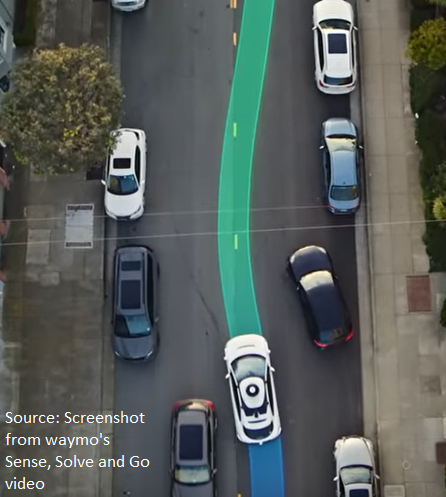
\includegraphics[scale=1]{1/waymo.png}
\caption{Waymo's L3 Data-Driven Agent}
\label{fig:waymo}
\end{center}
\end{figure}

\begin{figure}[h]
\begin{center}
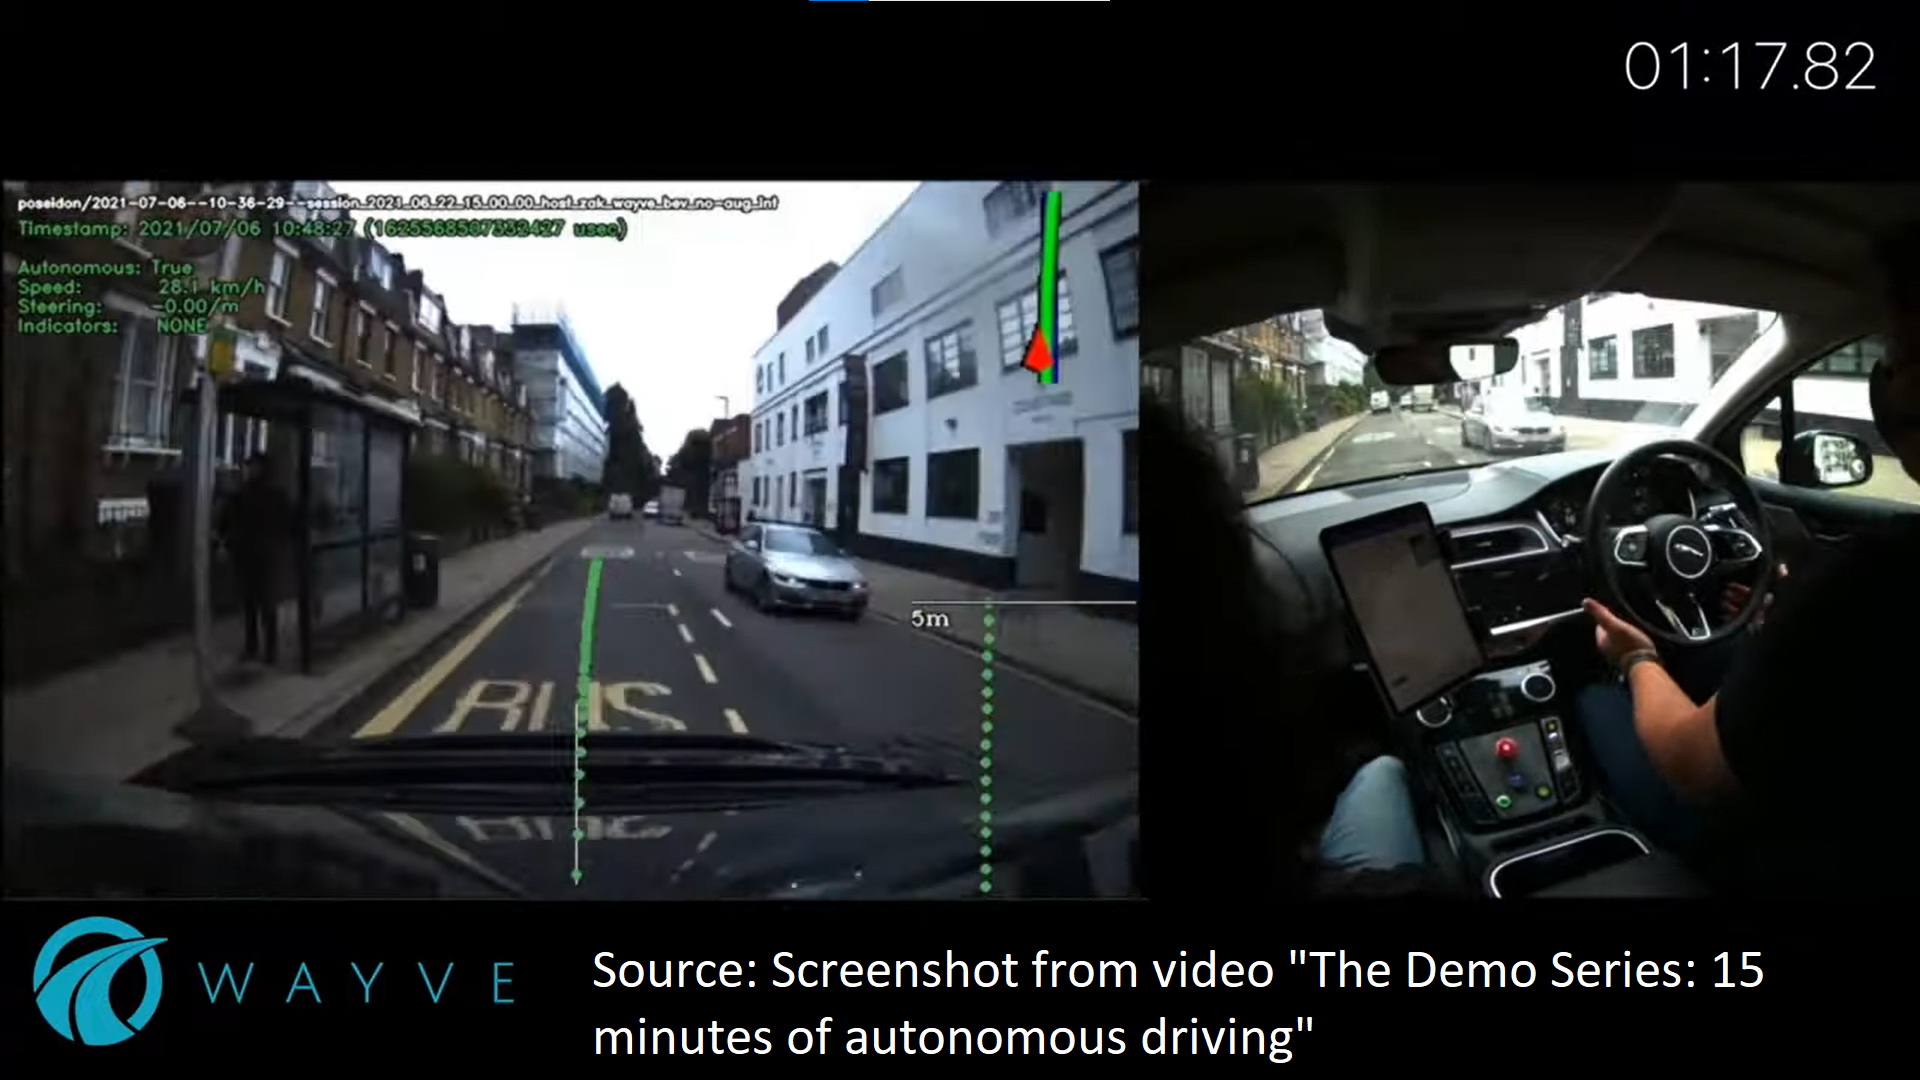
\includegraphics[scale=0.3]{1/wayve.png}
\caption{Wayve's L3 Data-Driven Agent}
\label{fig:wayve}
\end{center}
\end{figure}

\begin{figure}[h]
\begin{center}
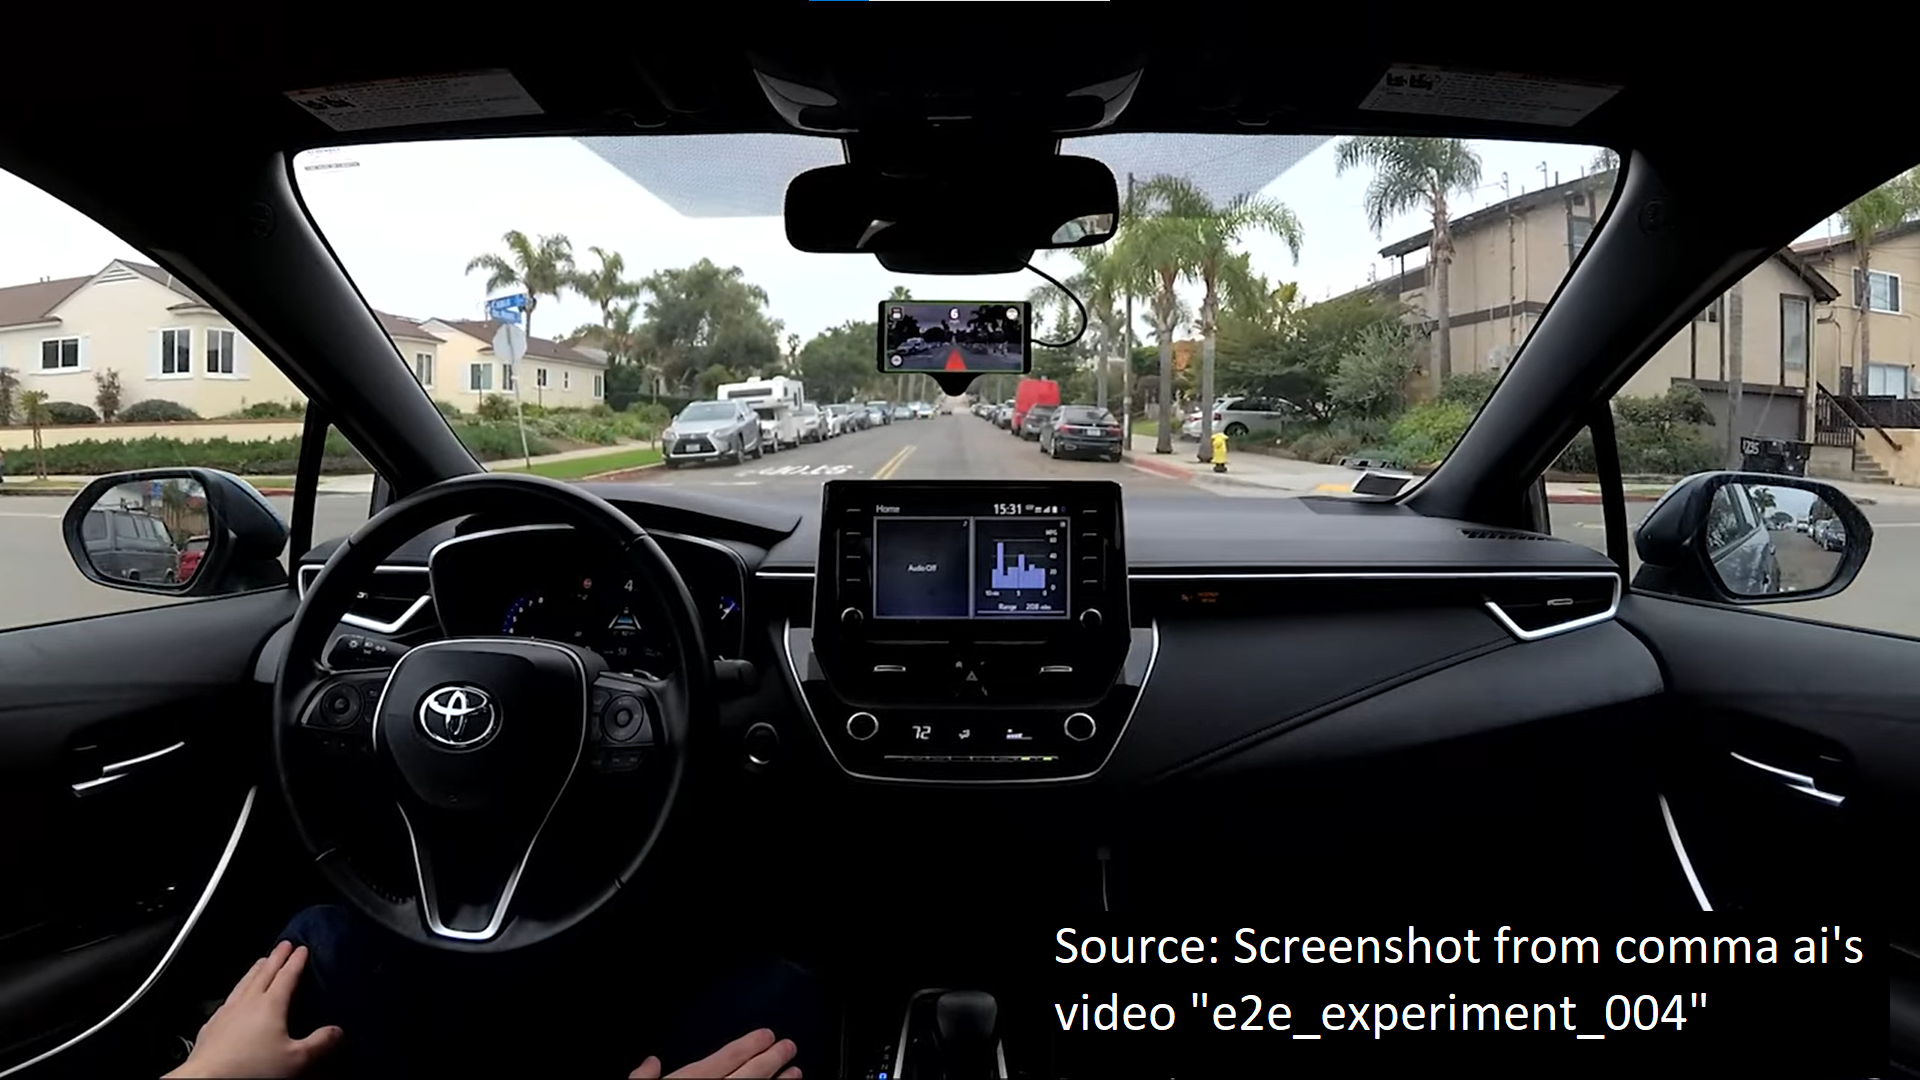
\includegraphics[scale=0.3]{1/comma.png}
\caption{Comma's L2 Data-Driven Agent}
\label{fig:comma}
\end{center}
\end{figure}

\begin{spacing}{1.5} 
\begin{sloppypar}
Research on Artificial Intelligence algorithms has rapidly progressed along with Big Data and advanced computational capabilities. AI-guided autonomous systems don't require any system-level knowledge and have great potential to optimize nonlinear systems in complex and dynamic environment. 
\end{sloppypar}
 \end{spacing}

 \begin{spacing}{1.5} 
 \begin{sloppypar}
 The Intelligent Vehicle industry is in a stand still despite of astonishing intellectual gains over the recent years. This is because SOTA Autonomous Driving technology only works reliably by overfitting on the distribution of data. The SOTA AD systems that are expert driver in ideal environment breakdown the minute it is introduced to out-of-distribution data. 
 \end{sloppypar}
  \end{spacing}


  \begin{spacing}{1.5} 
  \begin{sloppypar}
  The solution for dealing with out-of-distribution data is to incorporate knowledge-driven driving agents. With the recent advent of high-performing LLMs, implementation of knowledge-driven agents with zero-shot capabilities (meaning no fine-tuning or training the LLMs for specific downstream tasks) is feasible. 
  \end{sloppypar}
   \end{spacing}

\begin{spacing}{1.5} 
\begin{sloppypar}
In this work, we explore the use of AD task of planning as way to evaluate LLMs ability to use logical reasoning to make decisions that have short and long term effects. The AD task used in this work is an open-source gymnasium environment called 'HighwayEnv'.
\end{sloppypar}
 \end{spacing}
 
\begin{spacing}{1.5} 
\begin{sloppypar}
\section{TESTING}
Several companies that produce Intelligent Vehicles encountered accidents during testing or running. This has increased the demand for intelligent testing. Intelligent testing can identify cause of accidents and fix complications in Intelligent Vehicle systems \cite{chen2023milestones}.

There are 2 types of testing platforms. 1) Simulation Platforms and 2) Vehicles Platforms

\subsection{Simulation Platforms}
To model vehicle dynamics, tools such as 1) Carsim with ADAMS, 2) CARLA, 3) PreScan and 4) MATLAB or Simulink have been used by researchers for simulating car behaviour. Using simuluation platforms have the benefit of being able to create your own situations and test the model's behaviour in a collection of created situations.  

\subsection{Vehicles Platforms}
Some researchers use the simulation studies as first step for performance validation and conduct experimental for further validation. This is shown in the papers \cite{muller2005off} and  \cite{arifin2022steering}
\end{sloppypar}
 \end{spacing}

 
\begin{spacing}{1.5} 
\begin{sloppypar}
\section{PROBLEMS RELEVANT TO THE RESEARCH}
\begin{itemize}
    \item Lack of testing environment for LLMs with respect to Autonomous Driving planning task
    \item Lack of enough dynamic evaluation metrics 
\end{itemize}

\section{RESEARCH OBJECTIVES}
\begin{itemize}
    \item Providing a customizable platform for easy testing of LLMs Autonomous Driving planning capabilities in zero shot setting.
    \item Providing a Plug and Play dynamic evaluation metric
\end{itemize}
\section{OVERVIEW OF THE PROPOSED SYSTEM}
This work gives an interface for testing a LLM for the AD planning task. This work uses the autonomous driving environment "DuckieTown" to perform simple tasks using LLMs. The LLM chosen for this purpose is the "PHI-2" due to its small size and strong performance.
\end{sloppypar}
 \end{spacing}
 
 \begin{spacing}{1.5} 
\begin{sloppypar}
\section{ORGANIZATION OF THE REPORT}

This report is organized into 6 chapters, describing each part of the project with detailed illustrations and system design diagrams. \newline
\textbf{CHAPTER 2:} Literature Review reviews existing research, studies, and relevant literature related Autonomous Driving. Discusses the background, theories, and methodologies used by other researchers\newline 
\textbf{CHAPTER 3:} System Design describes the design of the project. Explains the architecture, components, algorithms, and any other technical details.\newline
\textbf{CHAPTER 4:} Implementation provides details about how the project was implemented. Discusses the tools, technologies, programming languages, and frameworks used.\newline
\textbf{CHAPTER 5:} Result and Analysis presents the results of the project. Analyzes the outcomes, compare them with expectations, and discuss any challenges faced during implementation.\newline
\textbf{CHAPTER 6:} Conclusion and Future Work summarizes the findings and draws conclusions. Discusses the significance of your work and its implications\newline
\end{sloppypar}
 \end{spacing}
% Chapter 2

\chapter{\uppercase{Literature Survey}} % Main chapter title
\label{ch:survey} % For referencing

\begin{spacing}{1.5} 
\begin{sloppypar}
\section{AUTONOMOUS DRIVING}
Autonomous Driving (AD) refers to the technology of making the vehicle capable of sensing the surrounding environment and operating without human intervention or involvement. Intelligent Vehicles (IV) refers to a vehicle that owns the above technology to enable partial or fully automated functions. \cite{chen2023milestones}

AD can be categorized as 3 modules:
\begin{itemize}
    \item Perception
    \item Planning
    \item Control
\end{itemize}

The Society of Automotive Engineers (SAE) provides a taxonomy with detailed definitions of vehicle driving automation systems. There are 6 levels, they are:
\begin{itemize}
    \item Level 0 (L0): No automation
    \item Level 1 (L1): Driver Assistance
    \item Level 2 (L2): Partial Driving Automation
    \item Level 3 (L3): Conditional Driving Automation
    \item Level 4 (L4): High Driving Automation
    \item Level 5 (L5): Full Driving Automation
\end{itemize}
% insert architecture here
\subsection{Perception}
The perception of IVs is the first and the foundational step which determines the performance of the next stages. The perception is done using sensors such as Radar, cameras, GNSS, Lidar, Ultrasonic, Lidar, etc. To reduce the probability of failure and uncertain variables intervening, multiple different sensors are generally used. 

\subsubsection{Lidar}
They support high resolution 3D point cloud, Larger and wider sensing range, Accurate object and distance detection and robust to lightning but have high cost, poor performance in harsh weather and produce a large amount of data. The Figure \ref{fig:lidar} shows the newest technology in Lidar sensor: silicone-based Lidar sensors. Silicone based Lidar sensor reduce the volume of the conventional Lidar sensor and achieve a monolith integration. This removes the moving parts of the conventional Lidar sensors and realises solid-state beam steering \cite{hu2023advances}. 

\begin{figure}[h]
\begin{center}
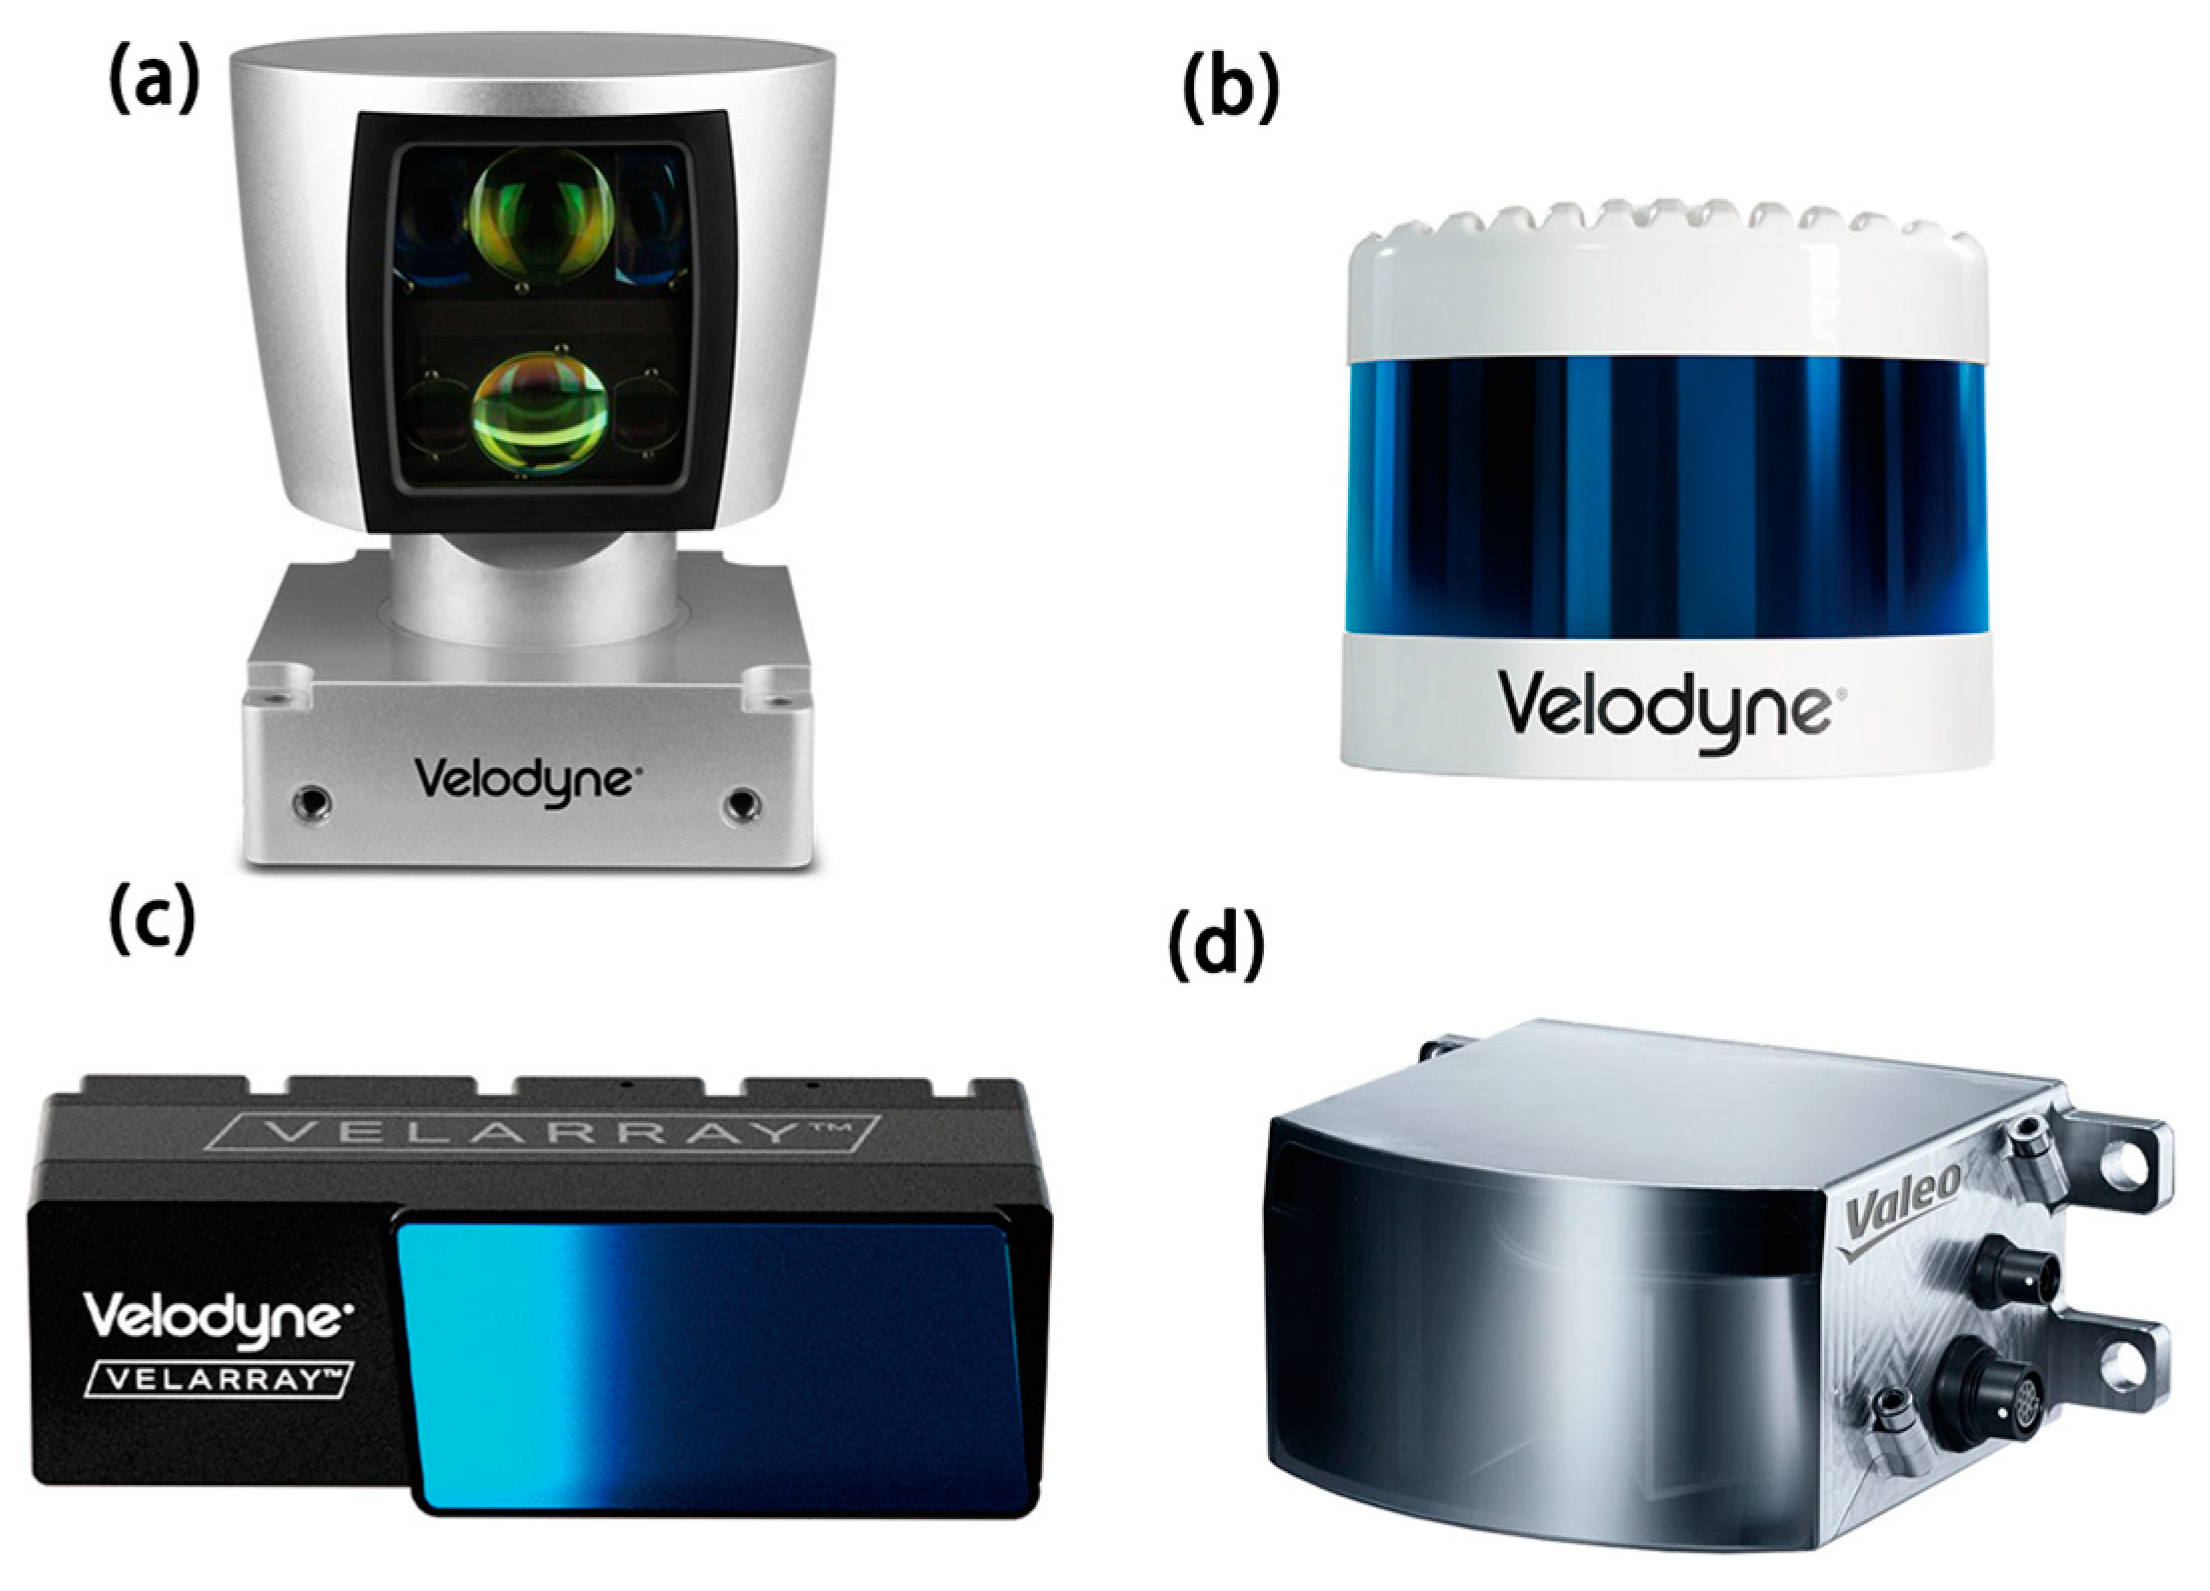
\includegraphics[scale=0.1]{2/lidar_Sensor.png}
\caption{Silicone-based Integrated Lidar Sensors in Intelligent Vehicles}
\label{fig:lidar}
\end{center}
\end{figure}

\subsubsection{Camera}
They are cost effective, support visual recognition and texture extraction but are easily affected by real world non-ideal environmental variables such as lighting and weather.

Multi-Object Tracking (MOT), an essential step in AD perception task, can be achieved by multiple cameras alone. Although, in practice, they are combined with Lidar and other sensors for SOTA performance. In the paper \cite{pereira2016self}, Akshay Rangesh et al utilize cameras and Lidar to achieve full-surround MOT using a modular design and also compares the results of different configurations such as number of cameras and positioning of cameras. Figure \ref{fig:camera} shows the full-surrond MOT using cameras. 

\begin{figure}[h]
\begin{center}
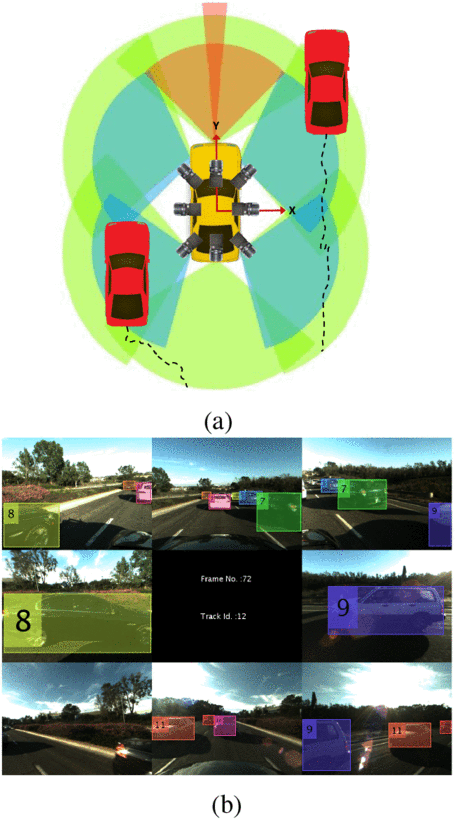
\includegraphics[scale=0.5]{2/camera.png}
\caption{Full-surround MOT using Cameras in Intelligent Vehicles}
\label{fig:camera}
\end{center}
\end{figure}
\subsubsection{Radar}
They support extreme long sensing range, are resilient to various external conditions but produce to little of data and cannot produce distinguishing features for targets.

Automotive radar have become more prominent due to its recent advancements in the radio-frequency (RF) CMOS technology that allows high-level radar on-chip integration. This lowers the cost of radar for mass production for consumers. But a disadvantage of mass produced consumer level radars are that they do no produce high spatial resolution. This can be mitigated by the multiple-input, multiple-output (MIMO) and cognitive approaches as discussed in this paper \cite{bilik2019rise}. Figure shows \ref{fig:radars} Radars using in Intelligent Vehicles. 

\begin{figure}[h]
\begin{center}
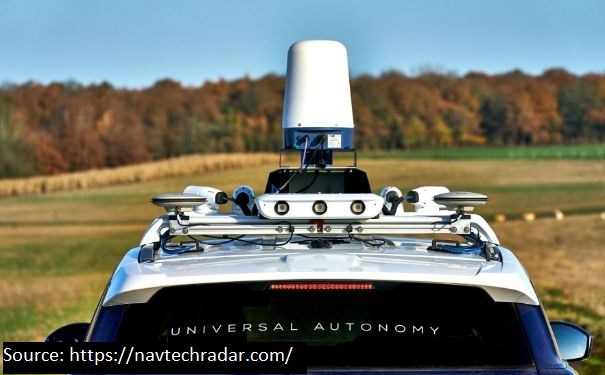
\includegraphics[scale=0.7]{2/radar.jpg}
\caption{Radars in Intelligent Vehicles}
\label{fig:radars}
\end{center}
\end{figure}

\subsubsection{GNSS}
They cost low, stable but have low accuracy, slow update frequency and require unobstructed view.

Modern Global Navigation Satellite Systems (GNSS) consists of four independent gloval satellite constellations delivering modernized signals at multiple civil frequencies. New ground monitoring infrastructure, mathematical models and internet services correct for errors in the GNSS signals at continent scale. Mass produced automotive grade receiver chipsets are available at low cost, size, weight and power (CSWaP). GNSS delivers better than lane-level accuracte localization with 99.99999\% integrity with over 95\% availability according to this paper \cite{joubert2020developments}. 
% \subsubsection{Ultrasound}
% They are Low cost, High accuracy for close range and resilient to adverse weather conditions but can only detect for short-ranges and don't work in high speeds.


\subsection{Planning}

Data-driven autonomous driving systems are characterized as modular tasks in a sequential order: Perception, Prediction and Planning. There exists standalone models for each task or one model with multiple different heads for each tasks. Yihan Hu et al \cite{hu2023planning} argue that all resources should be concentrated on the planning task as to not waste any resources unnecessarily. They optimize perception and prediction modules to primarily benefit the task of planning of self-driving cars. Figure \ref{fig:planning} depicts 3 types of Autonomous Driving designs, they are a) Separate models for different tasks, b) Multi-task learning scheme shares a backbone with divided task heads, c) End-to-end paradigm unites modules in perception and prediction.

\begin{figure}[h]
\begin{center}
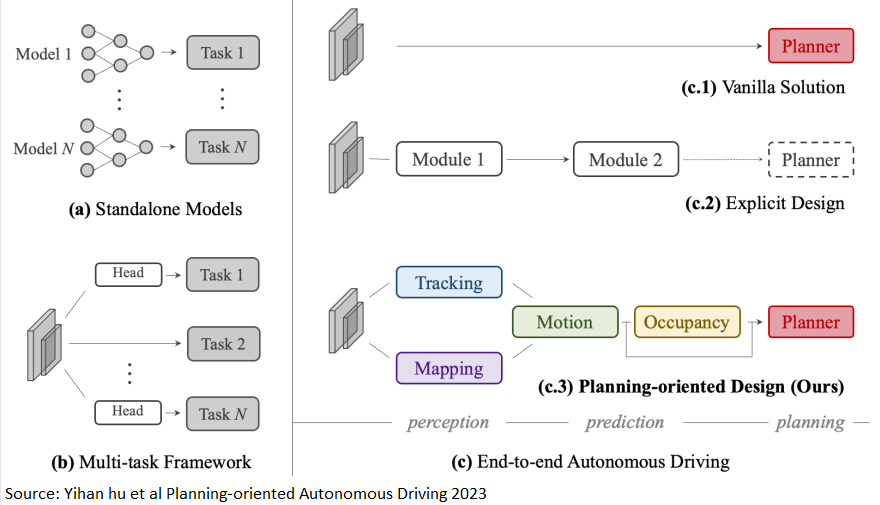
\includegraphics[scale=0.7]{2/hu2023Planning.png}
\caption{Planning-Oriented Autonomous Driving Design}
\label{fig:planning}
\end{center}
\end{figure}

 

\subsection{Control}
Vehicle control is an essential part of enhanced driver assistance. It includes tasks such as lateral stability control and driving at the limits for accident avoidance. There are two types of Motion control: 1) Longitudinal Vehicle Control which manages the acceleration of the vehicle through the vehicle's throttle and brake, and 2) Lateral Vehicle Control which controls the vehicle's position in the lane using the steering wheel. 

\subsubsection{Control Methodologies}
\textbf{PID Controller} or Proportional Integral Derivative Controller is a control loop mechanism employing feedback that is widely used in industrial control systems and variety of other applications requiring continuously modulated control according to Wikipedia.

In \textbf{Game-Theoretic Approaches} the vehicles are considered as players. Each player has a decision model which considers the game rules or traffic rules and other players to make it decisions. Since it considers what the other player will do, it is considered more reliable but has the drawback of being computationally intensive. 


\textbf{Fuzzy-Logic Control} is similar to PID controller, fuzzy-logic control does not require the mathematical model the mathematical model of the environment allowing the controller to adequately deal with nonlinear vehicle dynamics.

The principle of \textbf{MPC} or Model Predictive Control is to find a predictive motion solution over a longer horizon period by solving the problem at each sample tie and applying the first sequence of actions. In this way, MPC simulates a receding horizon control and changes the solution set to remain accurate to upcoming information.

\textbf{SMC} offers the capacity to adapt to unknown disturbances and matched uncertainties. 

\textbf{LPV Controller} is a linear controller and has been designed together with predictive control for lateral control and integrated system control.


\section{LARGE LANGUAGE MODEL}
LLMs are language models that are trained on large unsupervised datasets such as WebText. They are essential to the task of zero-shot task transfer for NLP task such as question and answering, machine translation, reading comprehension and summarization. Open-source of Open-access LLMs are model whose weights are publicly available for research and for some commercially also. LLMs are mad e up of transformers. GPT2 a predecessor of ChatGPT had size of 1.5 Billion parameters and was noted that it still didn't overfit meaning that it's performance can still be improved upon \cite{radford2019language}.
\subsection{OpenAI's GPT 3.5 And GPT 4}
OpenAI's ChatGPT-3.5, also known as GPT-3.5 Turbo, is a version of the Generative Pretrained Transformer (GPT) model that has been fine-tuned for chat applications. It is capable of understanding and generating natural language or code. This model was trained on an Azure AI supercomputing infrastructure and finished training in early 2022.
ChatGPT-3.5 Turbo has been optimized to perform better for specific use cases and run these custom models at scale. Early tests have shown that a fine-tuned version of GPT-3.5 Turbo can match, or even outperform, base GPT-4-level capabilities on certain narrow tasks. \cite{bahrini2023chatgpt}
% As for the reference paper, you can refer to the paper titled "ChatGPT: Applications, Opportunities, and Threats" submitted to arXiv.org on April 14, 2023. This paper provides a comprehensive examination of the applications, opportunities, and threats of ChatGPT in various domains. It also includes an experimental study comparing the performances of GPT-3.5 and GPT-4.

% \subsection{OpenAI's GPT 4}
\subsection{Llama And Llama2}
LLaMA and LLaMA 2 are collections of foundation language models developed by Meta AI. These models range in scale from 7 billion to 70 billion parameters.
LLaMA \cite{touvron2023llama} was trained on trillions of tokens using publicly available datasets exclusively. LLaMA-13B outperforms GPT-3 (175B) on most benchmarks, and LLaMA-65B is competitive with the best models, Chinchilla-70B and PaLM-540B.
LLaMA 2 \cite{touvron2023llama2} includes both pretrained and fine-tuned large language models (LLMs). The fine-tuned LLMs, called LLaMA 2-Chat, are optimized for dialogue use cases. LLaMA 2 outperforms other open-source chat models on most benchmarks.
These models are freely available for research and commercial use.

LLaMA introduces distinct innovations such as SwiGLU activation functions, rotary positional embeddings, root-mean-squared layer-normalization, and key-value caching. It also uses a zero-initialized attention mechanism with zero gating, which adaptively injects new instructional cues into LLaMA while effectively preserving its pre-trained knowledge.

\subsection{Mistral and Mixtral}
Mistral \cite{jiang2023mistral} is a 7-billion-parameter language model engineered for superior performance and efficiency. Mistral uses a Sliding Window Attention (SWA) mechanism. Each layer attends to the previous 4,096 hidden states. It also uses Grouped Query Attention (GQA), which allows for faster inference and lower cache size.
Mixtral is a Sparse Mixture of Experts model. Mixtral-8x7B outperforms GPT-3.5 using a technique called Mixture of Experts (MoE)
% \subsection{Mixtral}
% \subsection{OpenChat}

% \section{Data-driven IV}

% \subsection{Perception}
% \subsection{Planning}
% \subsection{Control}

\section{KNOWLEDGE DRIVEN DRIVING AGENTS USING LLM}
In this section, we will be looking at some recent papers that integrate LLMs to perform various autonomous driving task and give a review on how they do it. 
\pagebreak
\subsection{Working with Semantic Information}
To extract semantic information we use visual encoders. In Jinkyu Kim et. al. \cite{grounding} and Jinkyu Kim et. al. \cite{textual} the visual encoder is implemented using a Convolutional Neural Network.
Whereas Zhenhua Xu et. al. \cite{xu2023drivegpt4} uses a video tokenizer to take $N$ video frame. The tokenizer works by using a pretrained CLIP visual encoder to extract the features of $N$ input video frames. These tokens are then projected onto the text domain. Figure \ref{fig:driveGPT4} shows how this works.

Bu Jin et. al. \cite{jin2023adapt} also uses a video tokenizer but with Video Swin Transformer instead of CLIP to get the tokens.   

\begin{figure}[h]
\begin{center}
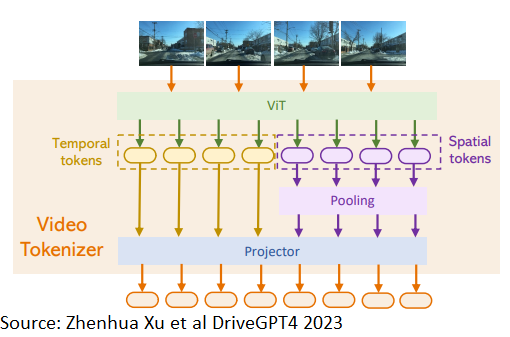
\includegraphics[scale=0.8]{2/DriveGPT4_1.png}
\caption{Architecture of Video Tokenizer}
\label{fig:driveGPT4}
\end{center}
\end{figure}

Zhenhua Xu et. al. \cite{xu2023drivegpt4} also use Llava (multimodal llm) and Yolov8 (real-time object detection) to generate prompts and give it to chatGPT to create a dataset for downstream task fine-tuning purpose. 

Long Chen et. al. \cite{chen2023driving} integrates numeric vector modality, a type of data frequently used in robotics to represent speed, actuator positions and distance measurements into the pretrained LLMs. This alleviates the problems of Visual Language Model's scaling problem. Figure shows the architecture of how this works.


\begin{figure}[h]
\begin{center}
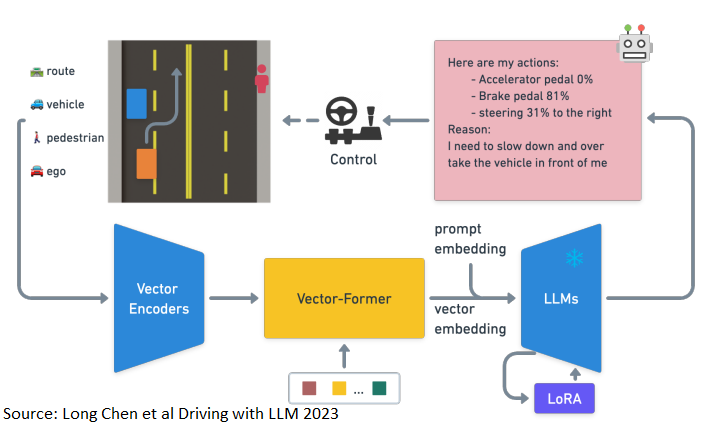
\includegraphics[scale=0.8]{2/vectorFusion.png}
\caption{Architecture with Vector Modality Instead of Visual Encoding}
\label{fig:vector}
\end{center}
\end{figure}


% \subsubsection{Multi-modal LLMs}


% There is an associated text encoder which encoders the text that describes the Image or video. 

\subsection{Autonomous Driving Tasks using LLMs}

In Licheng et. al. \cite{wen2023dilu}, an architecture for a knowledge-driven paradigm for Autonomous Driving System based on LLM that will interact with the environment to continuously evolve with a driver agent that recalls, reasons and reflects on it actions given a situation. The Figure \ref{fig:dilu} shows its architecture of a knowledge-driven driving agent using LLM.

\subsection{BDD-X Dataset}
Jinkyu Kim et. al. \cite{textual} uses Spatial, Temporal and Spatio-Temporal attention for vehicle control and explanation generation. It consists of 2 modules, 1) Vehicle Controller and 2) Explanation generator. The Figure \ref{fig:textual}

Jinkya Kim et. al. \cite{textual} includes the BDD-X dataset. It focuses on generating textual description and explanations such as the pair “Vehicle slows down” (description) and “Because it is approaching an intersection and the light is red” (explanation)". Figure \ref{fig:textual2} shows how the dataset is organized.  

\begin{figure}[h]
\begin{center}
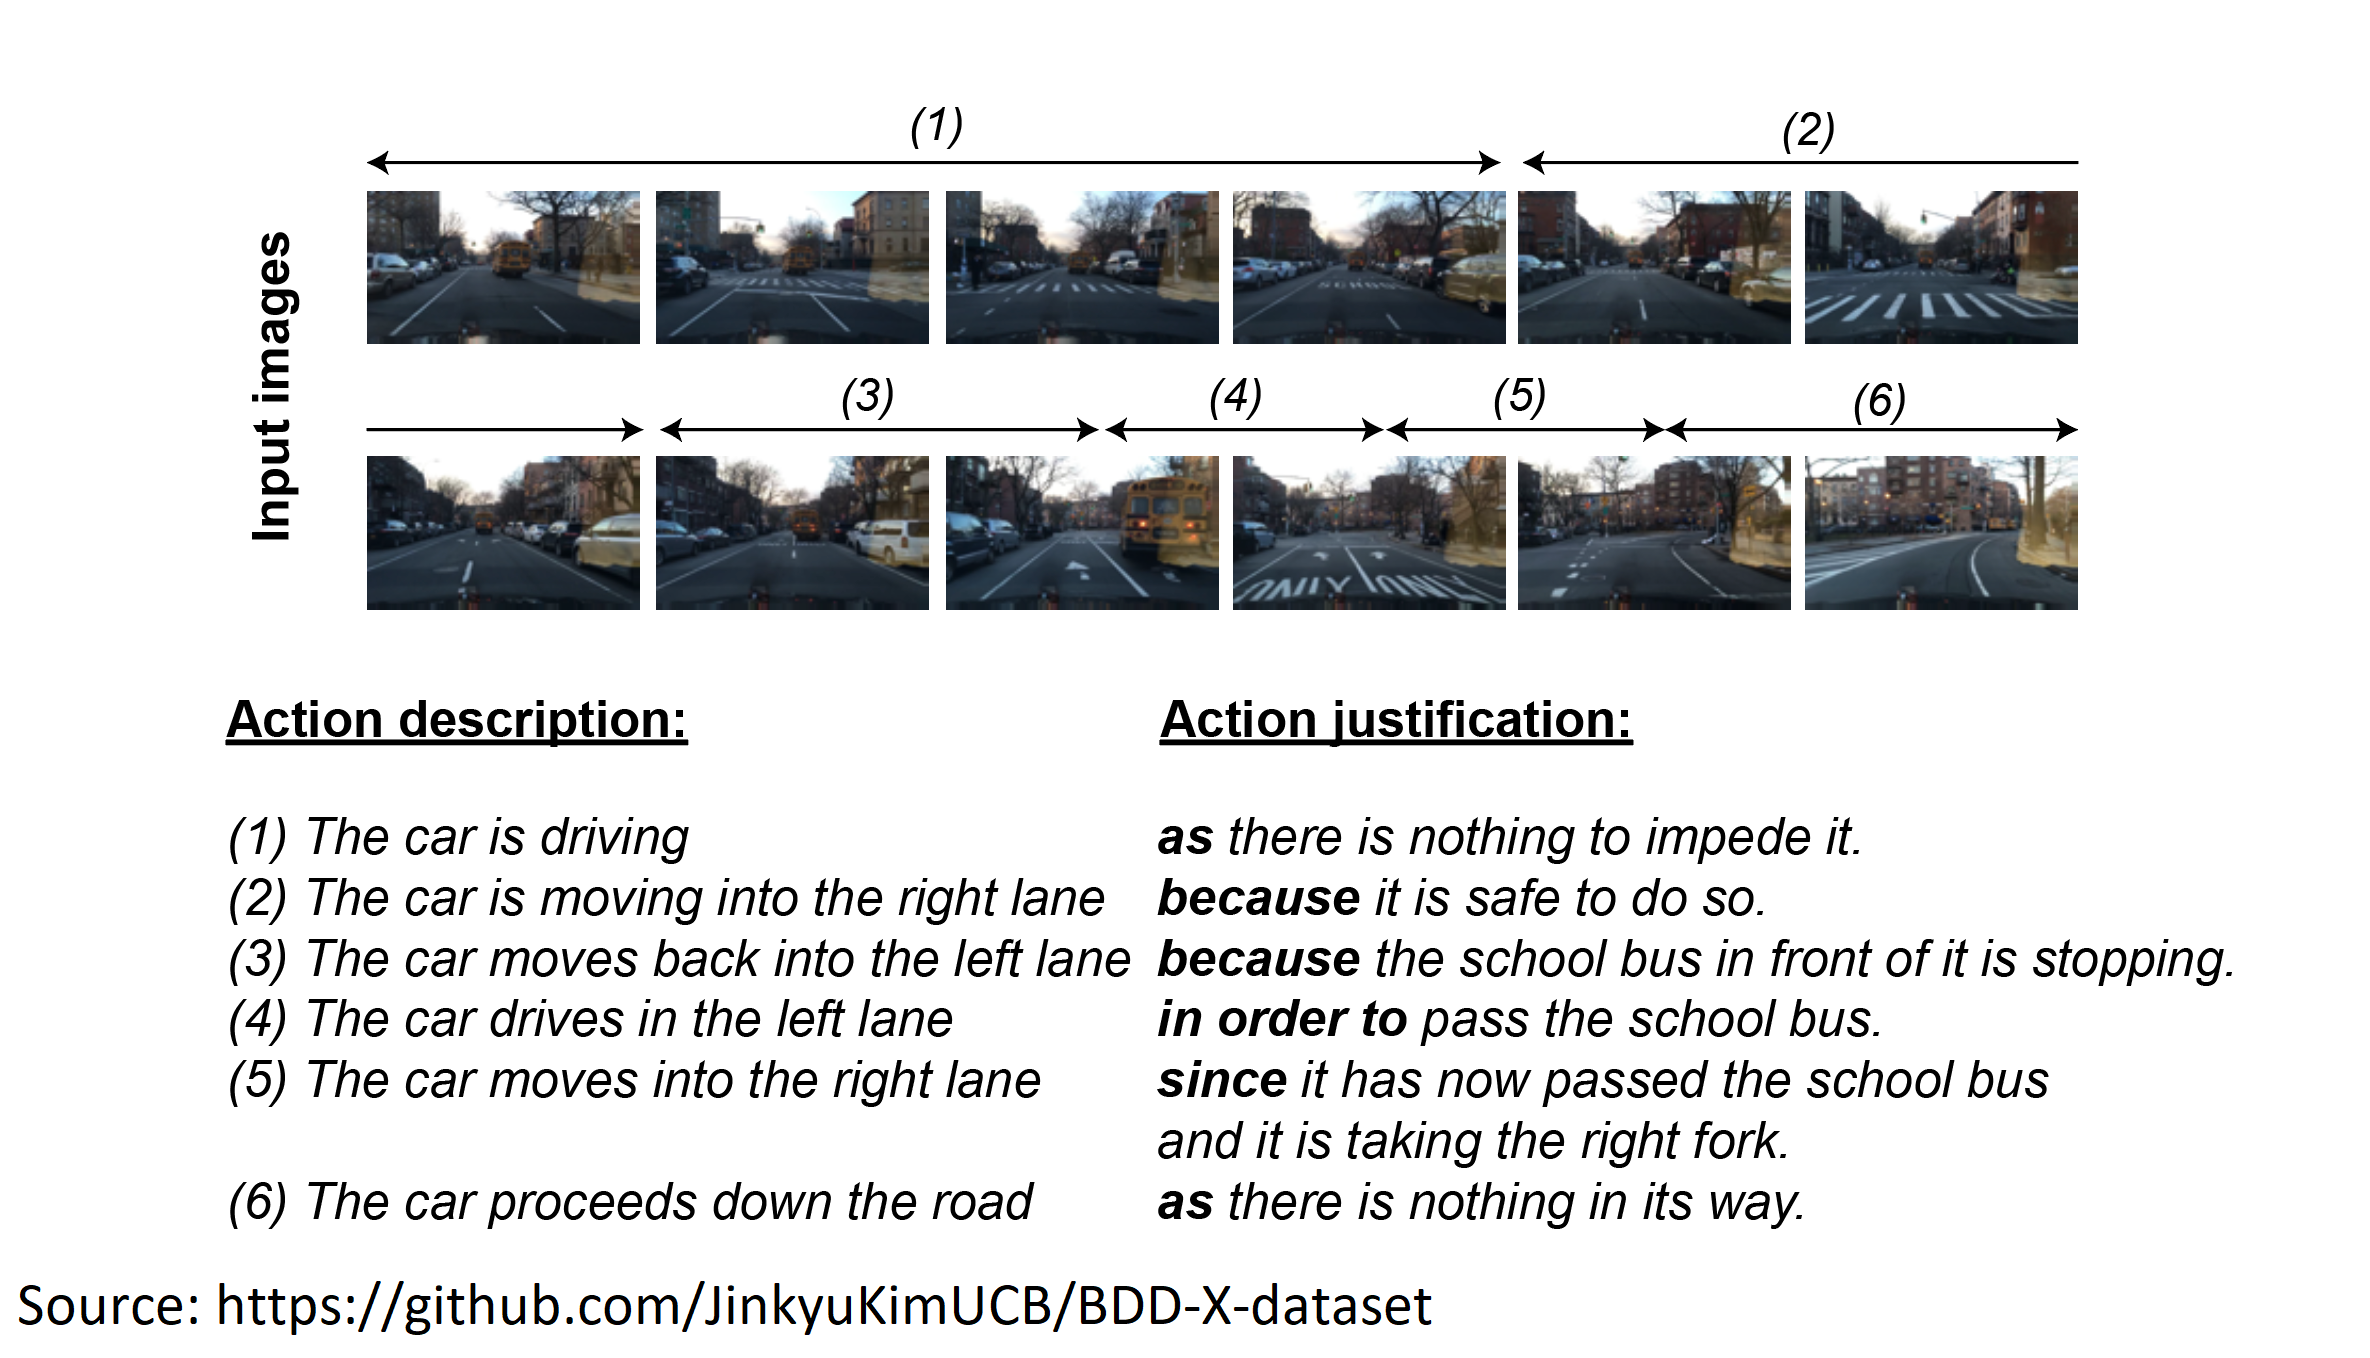
\includegraphics[scale=0.3]{2/textual_2.png}
\caption{BDD-X Dataset}
\label{fig:textual2}
\end{center}
\end{figure}

\begin{figure}[h]
\begin{center}
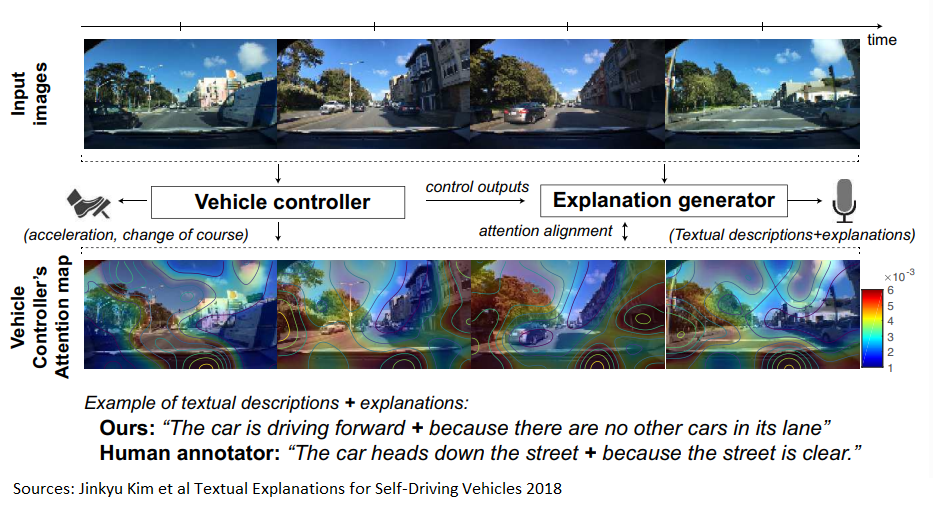
\includegraphics[scale=0.8]{2/textual_1.png}
\caption{Textual Explanations for Self-Driving Vehicles Overview}
\label{fig:textual}
\end{center}
\end{figure}

Bu Jin et. al. \cite{jin2023adapt} uses $T$ video frames as inputs (32 frames for best performance). It outputs are 1) control signal which is used to control the vehicle and 2) Text which consists of narration (what is happening?) and reasoning(why it is happening?). This work is similar to Jinkyu Kim et. al. \cite{textual} with few differences such as use of tranformers. The Figure \ref{fig:adapt} shows the architecture of Bu Jin et. al. \cite{jin2023adapt}.

\begin{figure}[h]
\begin{center}
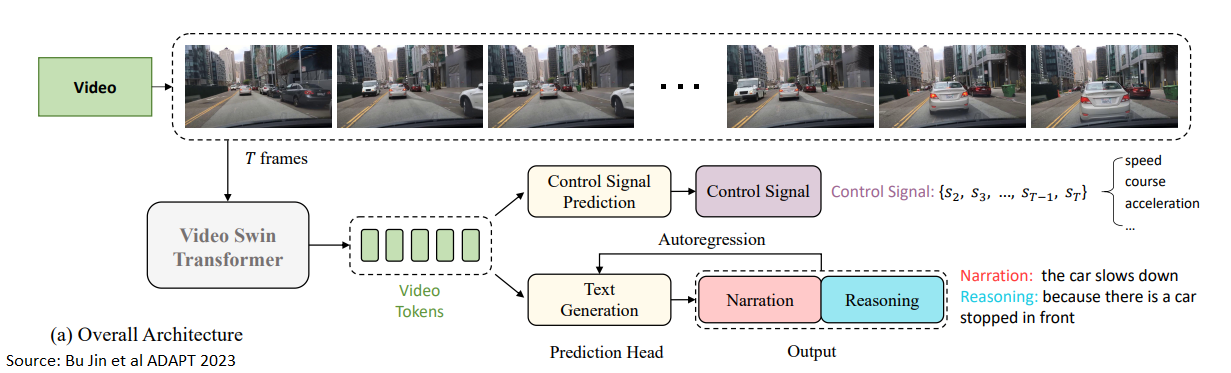
\includegraphics[scale=0.6]{2/ADAPT_1.png}
\caption{ADAPT Overview}
\label{fig:adapt}
\end{center}
\end{figure}

Zhenhua Xu et. al. \cite{xu2023drivegpt4} uses 8 video frames as inputs to predict the next viable actions to take as well as attain a reasonable understanding of its situation. Figure \ref{fig:driveGPT4_2} shows the work of Zhenhua Xu et. al. \cite{xu2023drivegpt4}.

\begin{figure}[h]
\begin{center}
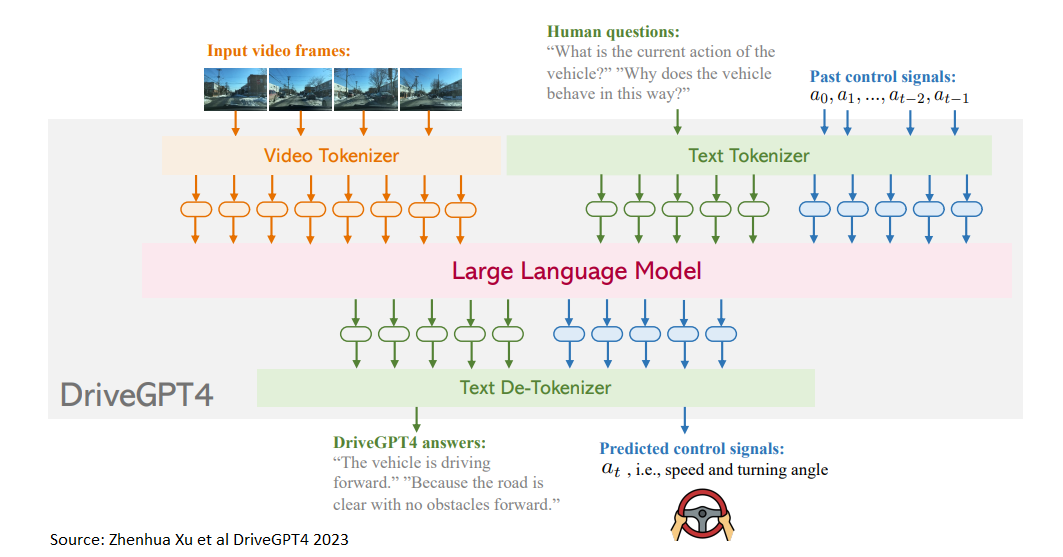
\includegraphics[scale=0.7]{2/DriveGPT4_2.png}
\caption{DriveGPT4 Overview}
\label{fig:driveGPT4_2}
\end{center}
\end{figure}


\begin{figure}[h]
\begin{center}
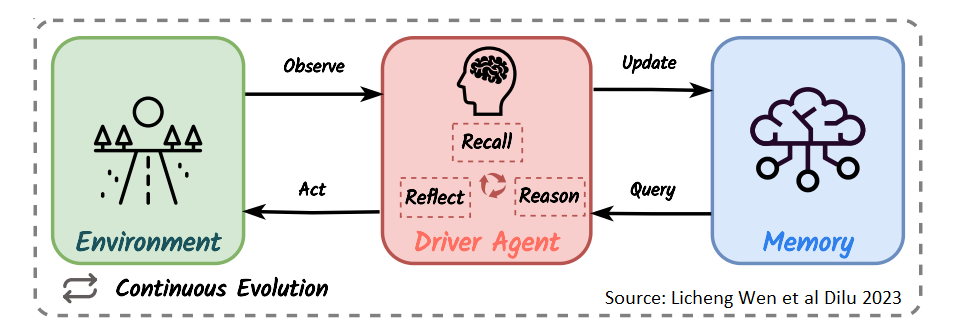
\includegraphics[scale=0.7]{2/Dilu_1.png}
\caption{A Knowledge-Driven Driving Agent Architecture using LLM}
\label{fig:dilu}
\end{center}
\end{figure}

This work is based on the Daocheng Fu et al \cite{fu2023drive}, GPT 3.5  observes its environment using perception tools and makes discrete decisions to control the ego vehicle. GPT 3.5 employs the ReAct strategy to plan actions and use tools to perceive its surroundings through a cycle of thought, action and observation. Figure \ref{fig:driving} shows the work of Doacheng Fu et al \cite{fu2023drive}.

\begin{figure}[h]
\begin{center}
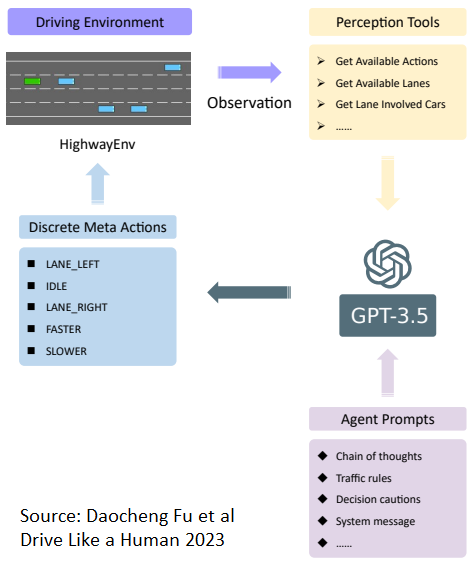
\includegraphics[scale=1.5]{2/DriveLikeHuman_1.png}
\caption{Driving like a Human}
\label{fig:driving}
\end{center}
\end{figure}
\end{sloppypar}
 \end{spacing}

 

% Chapter 3

\chapter{\uppercase{System Design}} % Main chapter title
\label{ch:chap3} % For referencing
\begin{spacing}{1.5} 
\begin{sloppypar}
There are 3 workflow for creating an Autonomous Driving Agent using this project
\begin{itemize}
    \item Data collection and annotation
    \item Building Vector Database
    \item Autonomous Driving Environment Interaction Loop
\end{itemize}

\begin{figure}[h]
\begin{center}
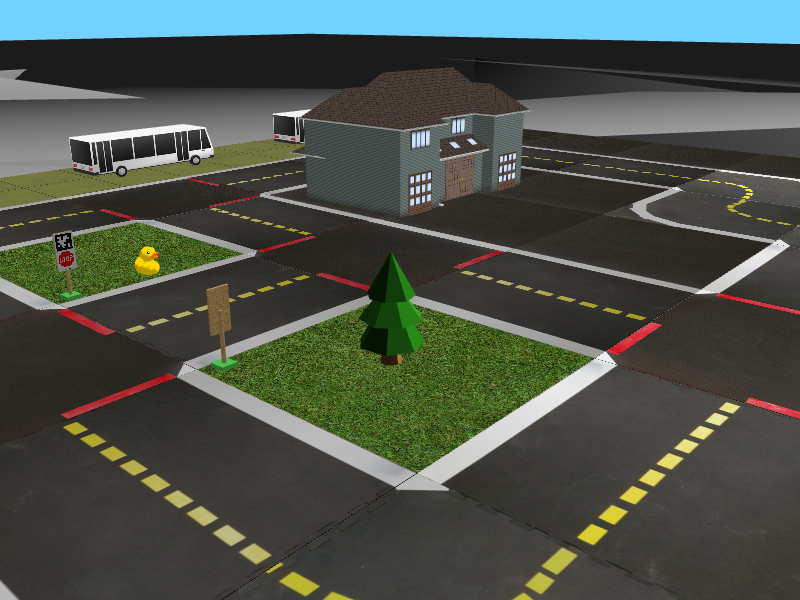
\includegraphics[scale=0.5]{3/duckieTown.png}
\caption{DuckieTown}
\label{fig:DuckieTown}
\end{center}
\end{figure}

% \subsection{4way}


\begin{sidewaysfigure}[h]
\begin{center}
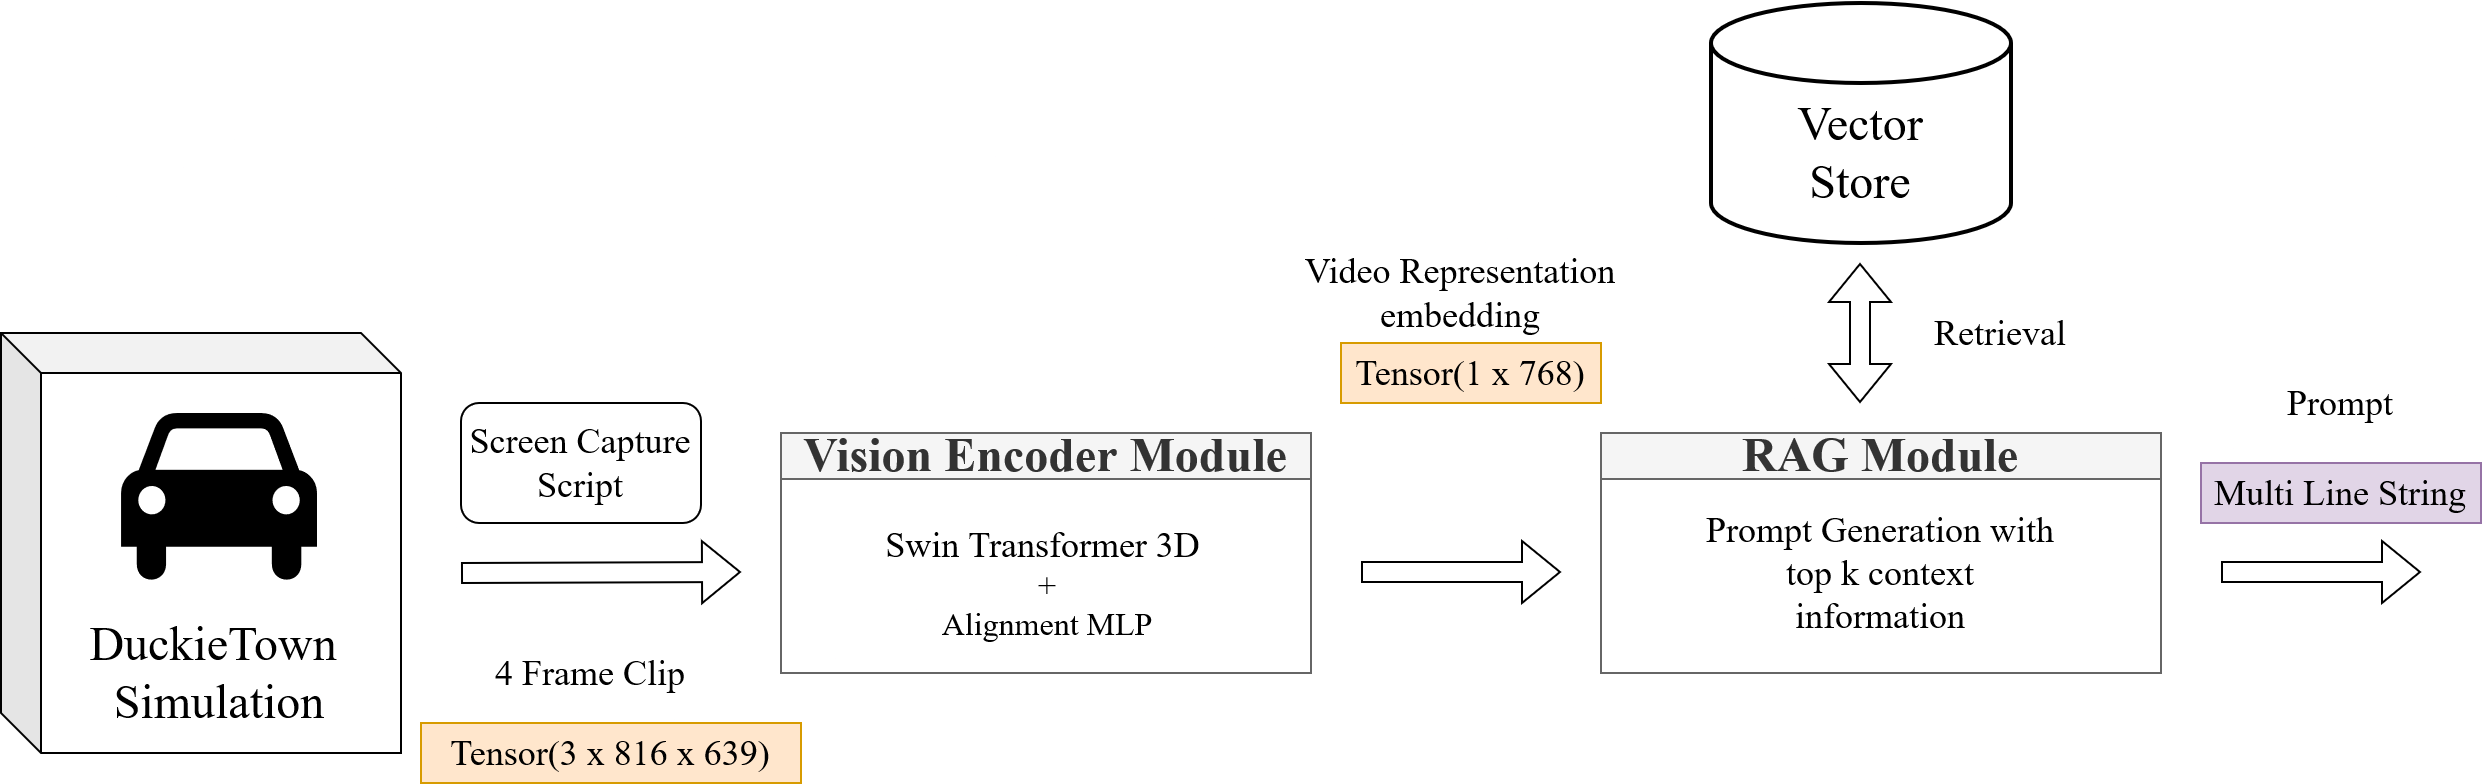
\includegraphics[scale=0.28]{3/retrieval_rag.png}
\caption{RAG Retrieval Architecture}
\label{fig:archi}
\end{center}
\end{sidewaysfigure}

\begin{sidewaysfigure}[h]
\begin{center}
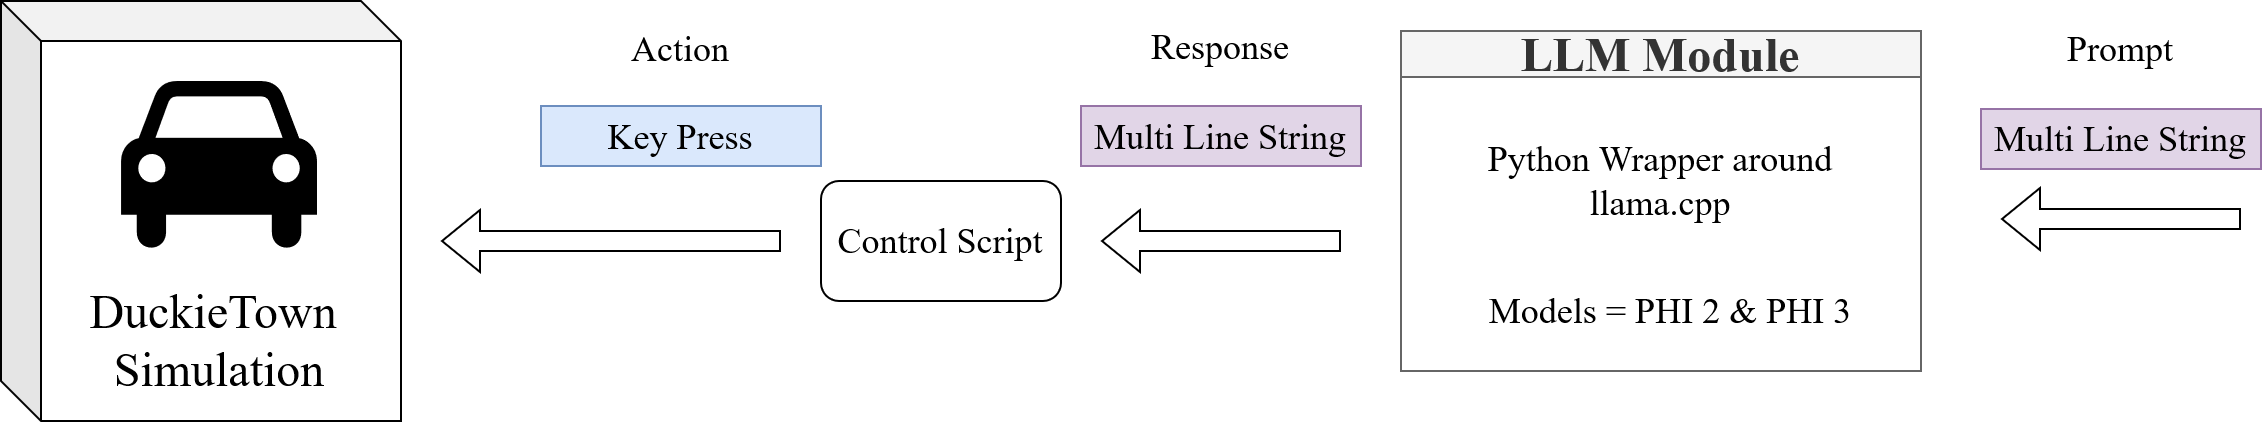
\includegraphics[scale=0.28]{3/rag generation.png}
\caption{RAG Generation Architecture}
\label{fig:rag_generation}
\end{center}
\end{sidewaysfigure}



\section{DATA COLLECTION TOOL}
The Data Collection tool module consists of 2 sub-modules. 
Data collection tools are indispensable in the realm of research and analysis, serving as the backbone for acquiring accurate and reliable data. These tools facilitate a systematic approach to gathering information, ensuring consistency and reducing biases that could compromise the integrity of the data. The significance of these tools extends across various domains, from business intelligence to scientific research, where they enable the extraction of meaningful insights from raw data. 

In the digital age, data collection tools have evolved to handle the vast amounts of information generated every second. They range from simple online surveys to complex analytics software, each designed to fulfill specific research needs. For instance, surveys are commonly used to collect quantitative data, while interviews and focus groups are tailored for qualitative insights. 

Moreover, the importance of data collection tools lies in their ability to transform disparate data points into coherent patterns and trends. This transformation is crucial for making informed decisions, developing strategies, and predicting future trends. In business, for example, data collection tools can reveal consumer behavior patterns, market trends, and operational inefficiencies, guiding strategic planning and competitive positioning.

In healthcare, data collection tools are used to track patient outcomes, improve treatment protocols, and manage public health initiatives. In education, they assist in evaluating student performance, curriculum effectiveness, and institutional policies. Similarly, in government, these tools support policy development, resource allocation, and service delivery.

The advent of big data and advanced analytics has further underscored the importance of robust data collection tools. They now must not only collect data but also ensure its quality, relevance, and timeliness. With the integration of artificial intelligence and machine learning, data collection tools are becoming smarter, capable of identifying patterns and anomalies that would otherwise go unnoticed.

In conclusion, data collection tools are vital for capturing the essence of the complex world around us. They empower researchers, analysts, and decision-makers with the clarity needed to navigate the intricacies of their respective fields. As we continue to advance technologically, the development and refinement of these tools will remain a critical focus, ensuring that our decisions are grounded in solid, empirical evidence.

\subsection{Recorder}
The data collection tool's recorder is used to procure the dataset required by the Autonomous Driving agent. The Data Collection tool captures small clips from a specific window. You can specific the window, the number of frames per second you are recording and number of frames per clip. You can run this data collection tool in the background and record the particular actions you perform.
\subsection{Data Annotation Tool}
The data annotation tool is used to annotate the recorded clips for the Autonomous Driving agent to use. This is required because the Autonomous Driving agent uses both textual and visual data to understand the semantic meaning of the visual data.

    


\section{RETRIEVAL AUGMENTED GENERATION}

Retrieval-Augmented Generation (RAG) represents a significant advancement in the field of natural language processing (NLP) and Artificial Intelligence (AI). It is a hybrid approach that combines the strengths of two distinct models: retrieval-based and generative. The retrieval component of RAG is responsible for sourcing relevant information from a vast knowledge base, which can include structured databases or unstructured text. This process ensures that the data used for generating responses is grounded in factual and authoritative content, thereby enhancing the reliability and accuracy of the output.

The generative component of RAG then takes this retrieved information and constructs coherent and contextually relevant text. This could be in the form of answers to questions, dialogue for chatbots, or even content for articles. By integrating these two components, RAG effectively addresses some of the limitations inherent in purely generative models, such as the production of outdated or inaccurate information, and the potential for bias and misinformation.

One of the key benefits of RAG is its ability to remain current and specific without the need for constant retraining of the model. This is particularly advantageous for applications requiring up-to-date information or domain-specific knowledge. Additionally, RAG can significantly reduce the computational and financial costs associated with training large language models (LLMs), as it leverages existing knowledge bases rather than relying solely on the data it was trained on.

In practical terms, RAG can be utilized across a wide range of NLP tasks. For instance, in an AI chatbot designed to provide medical information, RAG can retrieve the latest research and guidelines from medical databases to inform its responses, ensuring that users receive the most current and accurate information. Similarly, in content generation, RAG can pull from recent news articles or scientific papers to create content that is both informative and timely.

Moreover, RAG's flexibility allows it to adapt to various languages and domains, making it a versatile tool for global applications. Its architecture, which augments the capabilities of LLMs by adding an information retrieval system, provides developers with greater control over the generated text output. This control is crucial for maintaining the quality and trustworthiness of AI-generated content.

In conclusion, Retrieval-Augmented Generation is a transformative technology that enhances the capabilities of AI in understanding and generating human language. By combining retrieval and generation, RAG offers a more accurate, relevant, and versatile solution for a multitude of NLP applications, pushing the boundaries of what is possible in the realm of AI and machine learning.



To implement RAG, we need a Vector Store. This Vector Store must have efficient lookup time to find the top k similar context information. Algorithms like K-Nearest Neighbors can be employed here. In our Autonomous Driving agent, we go for a simple linear search for finding the top k similar clips. This is because we currently only have a small amount of data, so for this scenario highly efficient algorithms are not necessary. Moving forward, we will be implementing a more efficient and scalable vector database.


\section{TEXT GENERATION}



Text generation using Large Language Models (LLMs) represents a significant advancement in the field of natural language processing (NLP). These models, trained on vast datasets, have the ability to generate coherent and contextually relevant text that closely mimics human writing. The underlying architecture of LLMs, such as the Transformer model, enables them to capture the nuances of language through deep learning techniques. They utilize mechanisms like attention and context to generate text that is not only grammatically correct but also semantically rich.

The training process of LLMs involves unsupervised learning, where the model is exposed to large corpora of text and learns to predict the next word in a sequence, thereby understanding language patterns and structures. This process equips LLMs with a broad understanding of language, enabling them to perform a variety of tasks such as translation, summarization, and question-answering. Moreover, the adaptability of LLMs allows for fine-tuning on specific domains or styles, enhancing their versatility.

One of the most remarkable aspects of LLMs is their ability to generate creative content. Whether it's composing poetry, writing stories, or even creating code, LLMs can produce original content that often requires a second glance to distinguish from that written by humans. This capability has opened up new possibilities in content creation, where LLMs can assist in drafting articles, generating dialogue for characters in games, or providing educational content.

However, the use of LLMs also raises important ethical considerations. The potential for generating misleading information or biased content is a concern that developers and users must address. Ensuring that LLMs are used responsibly involves incorporating checks and balances to prevent the dissemination of harmful content. Additionally, the environmental impact of training and running these large models is a subject of ongoing discussion, prompting a search for more efficient and sustainable methods.

In conclusion, text generation using LLMs is a rapidly evolving technology with immense potential. Its applications span across various industries, revolutionizing the way we interact with and produce written content. As the technology continues to advance, it will be crucial to navigate the challenges it presents to maximize its benefits for society.

There are many methods to save and load models. Recent popular format for saving and loading LLMs is called GGUF. With GGUF, you do not need to load the tokenizer, embedding layer and transformer seperately. Instead, all of it is saved as a single file. GGUF format is most popular to save quantized Large Language Models.

\section{VISION ENCODER}

The vision encoder must be able to understand spatio temporal context information between the sequence of frames. These encoded values must then by aligned with the embedding of description of the video. This alignment is necessary as the final embeddings  of the vision encoder along with prompt embeddings are used as query to find the top k similar clips in the RAG methodology.  

The vision transformer cannot get the entire sequence of image as input. It has to be split into patches. Then encoded with patch encoding and positional encoding. 

The Video Swin Transformer represents a significant advancement in the field of computer vision, particularly in the encoding of video data. It is a model that builds upon the Swin Transformer architecture, which is designed for image domain, to effectively handle video inputs. The key innovation of the Video Swin Transformer lies in its ability to capture the temporal dynamics of video data, which is crucial for tasks such as action recognition and scene understanding.

In mathematical terms, the Video Swin Transformer operates on 3D patches extracted from the input video. These patches are then processed through a series of Transformer layers that model the relationships between different patches. The Transformer layers use self-attention mechanisms, which can be represented mathematically as:

$$
\text{Attention}(Q, K, V) = \text{softmax}\left(\frac{QK^T}{\sqrt{d_k}}\right)V
$$

Here, \( Q \), \( K \), and \( V \) represent the query, key, and value matrices, respectively, which are derived from the input patches. The term \( d_k \) denotes the dimensionality of the key vectors, and the softmax function is applied to the rows of the matrix resulting from \( QK^T \).

The Video Swin Transformer introduces a hierarchical structure that allows it to handle the large-scale nature of video data efficiently. This is achieved by partitioning the video into non-overlapping 3D patches and then applying self-attention within local windows. As the layers go deeper, the windows are merged hierarchically, increasing the receptive field and enabling the model to capture more global information. The hierarchical nature of the model can be expressed as:

$$
\text{Swin}(x) = \text{W-MSA}(\text{LN}(x)) + x
$$

$$
\text{Swin}(x) = \text{SW-MSA}(\text{LN}(\text{Swin}(x))) + \text{Swin}(x)
$$

In the above equations, \( \text{W-MSA} \) and \( \text{SW-MSA} \) refer to the window-based multi-head self-attention and shifted window multi-head self-attention operations, respectively. \( \text{LN} \) denotes layer normalization, and \( x \) is the input to the respective layer.

The adaptability of the Swin Transformer to video tasks is further enhanced by its ability to leverage pre-trained image models, which provides a rich initialization that benefits video understanding. The Video Swin Transformer has demonstrated state-of-the-art performance on various video recognition benchmarks, making it a powerful tool for video analysis applications.


The patch encoding is converting a patch into a linear array. Patch encoding in vision transformers is a pivotal step in processing images for machine learning tasks. It involves the division of an image into fixed-size patches and then encoding these patches into a latent space that can be used for further processing by the transformer model. Mathematically, this process can be represented as follows: given an image \( X \in \mathbb{R}^{H \times W \times C} \), where \( H \), \( W \), and \( C \) represent the height, width, and number of channels of the image respectively, the image is divided into \( N \) patches each of size \( P \times P \times C \). Each patch is then flattened into a vector of size \( P^2 \times C \), and these vectors are linearly projected into a \( D \)-dimensional space using a trainable embedding matrix \( E \in \mathbb{R}^{(P^2 \cdot C) \times D} \). The mathematical formula for this encoding is \( z = E \cdot \text{vec}(x_p) \), where \( x_p \) is the flattened patch vector and \( z \) is the resulting encoded patch vector.

This encoding process is crucial because it allows the model to handle images of varying sizes and reduces the computational complexity compared to processing the entire image at once. The encoded patches are then fed into the transformer encoder, which uses self-attention mechanisms to capture the global dependencies between patches. The positional information of each patch is also important, as it helps the model to understand the spatial structure of the image. This is often incorporated through positional encodings that are added to the patch encodings before they are input to the transformer model.

The use of patch encoding in vision transformers represents a significant shift from the traditional Convolutional Neural Networks (CNNs) that dominated image processing tasks. Unlike CNNs, which apply filters to overlapping regions of the image, patch encoding treats each patch independently until the self-attention mechanism in the transformer model allows for interaction between them. This approach has shown great promise in various computer vision tasks, offering a more flexible and powerful way to model the complex relationships present in visual data. The mathematical rigor and the ability to capture long-range dependencies make vision transformers, powered by patch encoding, a cutting-edge tool in the field of machine learning and artificial intelligence.


The positional encoding is just to ensure that each position is differentiable by the transformer. This is down by concatenating a small random number to each of the patch encoding. 
Positional encoding plays a crucial role in vision encoding, particularly in the context of neural networks that deal with sequential data. In the absence of inherent sequential information within the input data, positional encodings are used to provide the model with the notion of the order of the elements. This is particularly important in models like Transformers, which, unlike RNNs, do not process data in sequence. The mathematical formulation of positional encoding typically involves a set of functions that map a position in the sequence to a high-dimensional space of real numbers. For instance, in the Transformer model, the positional encoding is added to the input embeddings at the bottom of the model architecture. The functions used for this purpose are often sinusoidal, as they can allow the model to easily learn to attend by relative positions, due to the fact that for any fixed offset \( k \), \( \sin(x+k) \) and \( \cos(x+k) \) can be represented as a linear function of \( \sin(x) \) and \( \cos(x) \). The standard positional encoding formula in a Transformer is given by:

$$
PE_{(pos,2i)} = \sin\left(\frac{pos}{10000^{2i/d_{model}}}\right)
$$

$$
PE_{(pos,2i+1)} = \cos\left(\frac{pos}{10000^{2i/d_{model}}}\right)
$$

where \( pos \) is the position, \( i \) is the dimension, and \( d_{model} \) is the dimensionality of the model's output space. This encoding can be extended to two-dimensional space, which is particularly useful for vision tasks. In this case, the positional encoding would take into account both the x and y coordinates of the position in the image. The 2D positional encoding can be formulated as:

$$
PE_{(x,y,2i)} = \sin\left(\frac{x}{10000^{2i/d_{model}}} + \frac{y}{10000^{2i/d_{model}}}\right)
$$

$$
PE_{(x,y,2i+1)} = \cos\left(\frac{x}{10000^{2i/d_{model}}} + \frac{y}{10000^{2i/d_{model}}}\right)
$$

This approach allows the model to understand the relative positioning of features in an image, which is essential for tasks such as image recognition, segmentation, and object detection. The use of positional encoding in vision encoding ensures that spatial hierarchies and relationships between different parts of the image are maintained and understood by the neural network, leading to more accurate and effective models for visual data processing.

The pre-trained vision transformer must have been trained with modality used in our work, i.e video without audio. This is to ensure that vision transformer produces useful and meaningful outputs. 

The output embedding from the vision transformer is then passed through Multi-Layered Perceptron. The purpose of this MLP is to take the vision transformer output and transform it into the embeddings of the video description embeddings. By doing this, we have built a vision encoder that takes 3 frames input and returns embedding vector that is close to the embedding vector that represents the video description. 

The alignment head is MLP with GELU activation function.

A Multi-Layer Perceptron (MLP) is a class of feedforward artificial neural network (ANN) that consists of at least three layers of nodes: an input layer, a hidden layer, and an output layer. Except for the input nodes, each node is a neuron that uses a nonlinear activation function. MLP utilizes a supervised learning technique called backpropagation for training. 

The nodes of the intermediate or hidden layers typically use a sigmoid function as their activation function, represented by the formula $$\sigma(x) = \frac{1}{1 + e^{-x}}$$ where \(x\) is the input to a neuron. This function introduces non-linearity to the model, allowing the network to learn more complex tasks.

For a given input vector \(X\), the output \(Y\) of a neuron is calculated using the weighted sum of the inputs, including a bias term, followed by an activation function. This can be represented as $$Y = \sigma(\sum_{i=1}^{n} w_i x_i + b)$$ where \(w_i\) represents the weight associated with the \(i\)-th input \(x_i\), and \(b\) is the bias.

The learning process involves adjusting these weights and biases to minimize the error in predictions. The error is quantified using a loss function, such as the mean squared error for regression tasks, given by $$E = \frac{1}{2}\sum_{i=1}^{n} (y_i - \hat{y}_i)^2$$ where \(y_i\) is the true value and \(\hat{y}_i\) is the predicted value by the model.

During backpropagation, the derivative of the error with respect to the weights is computed to update the weights in the direction that minimizes the error. This involves calculating the gradient of the loss function, which, for the mean squared error and sigmoid activation, can be expressed as $$\frac{\partial E}{\partial w_i} = (y_i - \hat{y}_i) \cdot \sigma'(\hat{y}_i) \cdot x_i$$ where \(\sigma'(\hat{y}_i)\) is the derivative of the activation function.

MLPs are widely used for pattern recognition, classification, and regression tasks. Their ability to model complex non-linear relationships makes them powerful tools in the field of machine learning. However, they can be prone to overfitting and may require techniques such as regularization and dropout to generalize better to unseen data. Despite these challenges, MLPs remain a fundamental building block in the architecture of deep learning models.

The Gaussian Error Linear Unit (GELU) is a type of activation function that is used in the field of neural networks, particularly in deep learning models. It combines properties of both the rectified linear unit (ReLU) and the normal distribution function, which allows it to model complex functions more effectively than traditional activation functions. The GELU function is defined mathematically as:

$$ GELU(x) = x \cdot \Phi(x) $$

where \( x \) is the input to the activation function, and \( \Phi(x) \) is the cumulative distribution function of the standard normal distribution. The formula for \( \Phi(x) \) is given by:

$$ \Phi(x) = \frac{1}{2} \left[1 + \text{erf}\left(\frac{x}{\sqrt{2}}\right)\right] $$

Here, \( \text{erf} \) represents the Gauss error function, which is a non-elementary function that cannot be expressed in terms of elementary functions. It is defined as:

$$ \text{erf}(x) = \frac{2}{\sqrt{\pi}} \int_{0}^{x} e^{-t^2} dt $$

The GELU activation function has been found to perform well in practice and is particularly useful in transformer models, such as those used in natural language processing tasks. It allows the network to learn to make more nuanced decisions about when to activate neurons, leading to improved model performance on a variety of tasks. The GELU function is smoothly non-linear when \( x \) is small, and approximately linear when \( x \) is large, which helps to mitigate the vanishing gradient problem that can occur with other activation functions like the sigmoid or hyperbolic tangent functions. This characteristic makes GELU an attractive choice for researchers and practitioners in the field of machine learning.



\begin{figure}[h]
\begin{center}
\includegraphics[scale=0.26]{3/Dissertation II_Video_Encoder.png}
\caption{Video Encoder}
\label{fig:Video Encoder}
\end{center}
\end{figure}

\begin{figure}[h]
\begin{center}
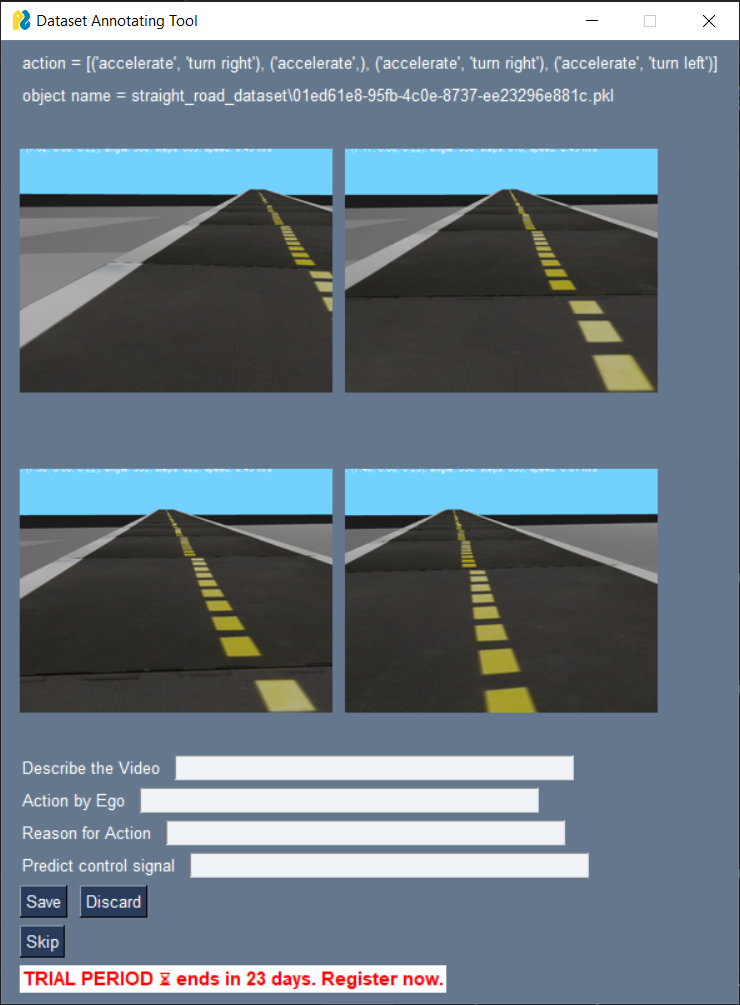
\includegraphics[scale=0.5]{3/Data Annotation.png}
\caption{Dataset Annotator}
\label{fig:Dataset Annotator}
\end{center}
\end{figure}
\end{sloppypar}
 \end{spacing}

 
% Chapter 4

\chapter{\uppercase{IMPLEMENTATION}} % Main chapter title
\label{chap4} % For referencing

\begin{spacing}{1.5} 
\begin{sloppypar}

In this chapter, we will discuss the implementation details of Autonomous Driving agent.
\section{ENVIRONMENT}

In fig. \ref{fig:4way}, you can see the a different map. There are 10 such different maps in the Duckietown simulator. We can built custom maps too. In fig. \ref{fig:loop_dyn_duckiebots}, you can see cart. This cart is a dynamic object (It moves as time passes).

DuckieTown Simulator is an innovative educational platform that merges the concepts of autonomous vehicles and gamified learning. Originating from the DuckieTown project, a university-led initiative for teaching robotics and artificial intelligence, the simulator provides a virtual environment where users can experiment with self-driving car algorithms. It is built on the Gym-Duckietown environment, which is a high-fidelity simulator written in Python and OpenGL, offering a customizable and interactive platform for users to test and develop their autonomous driving solutions.

The simulator is designed to reflect the complexities of real-world driving within a controlled setting, allowing for the testing of navigation, object detection, and control systems without the risks associated with physical vehicles. This is particularly useful for educational purposes, where students can learn about the intricacies of robotics software and hardware interaction in a safe and repeatable environment. The DuckieTown Simulator also serves as a research tool, providing a detailed and scalable environment to test advanced algorithms and behaviors before deploying them in real-world scenarios.

One of the key features of the DuckieTown Simulator is its integration with the Robot Operating System (ROS), which is a flexible framework for writing robot software. This integration allows for a seamless transition from simulation to real-world application, as the same code base can be used in both virtual and physical Duckiebots. The simulator supports various experiments, including reinforcement learning, where agents can be trained to navigate through the DuckieTown with the goal of reaching a destination efficiently while obeying traffic rules and avoiding obstacles.

Moreover, the DuckieTown Simulator is not just a tool for individual learning but also facilitates collaborative projects and competitions. It enables users from around the globe to participate in challenges that test the limits of their coding and problem-solving skills in a fun and engaging way. The simulator's open-source nature encourages community contributions, leading to continuous improvements and updates that enhance its capabilities and educational value.

In conclusion, the DuckieTown Simulator represents a significant advancement in the field of robotics education and research. It provides a bridge between theoretical knowledge and practical application, fostering a deeper understanding of autonomous systems. By offering a realistic and accessible platform, it empowers enthusiasts, students, and researchers alike to explore the future of mobility and autonomy. The simulator's contribution to the democratization of robotics education cannot be overstated, as it lowers the barriers to entry and allows a wider audience to engage with cutting-edge technology.
\begin{figure}
    \centering
    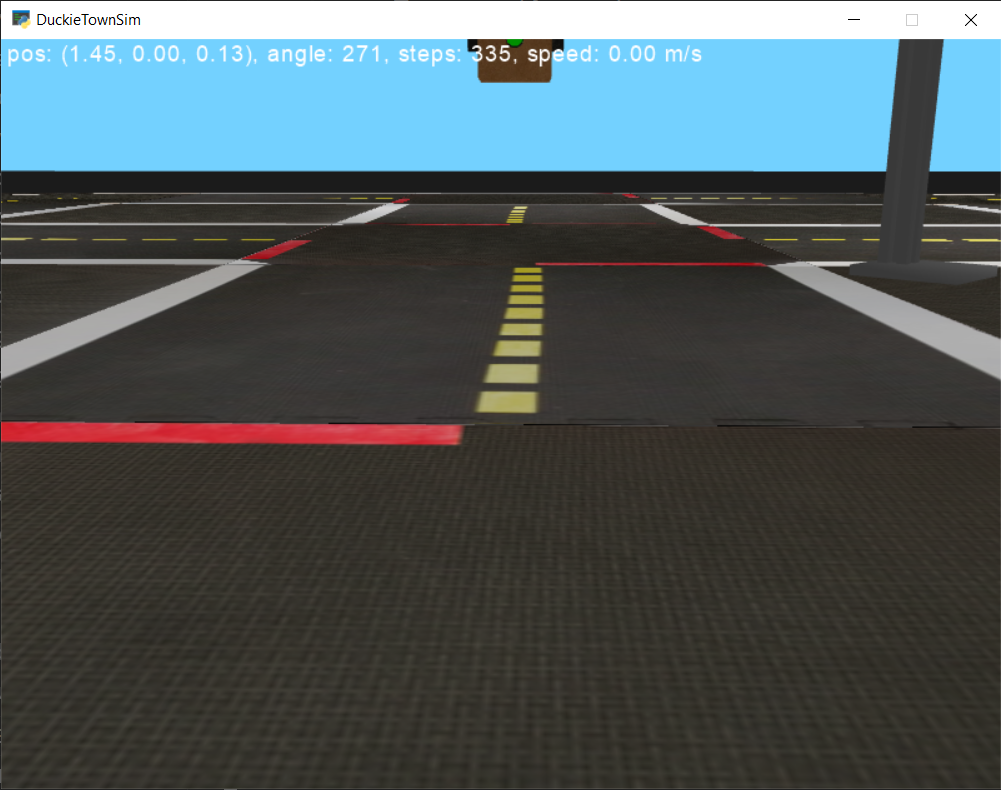
\includegraphics[width=1\linewidth]{4/4way.png}
    \caption{4way Environment}
    \label{fig:4way}
\end{figure}

% \subsection{loop\_dyn\_duckiebots}
\begin{figure}
    \centering 
    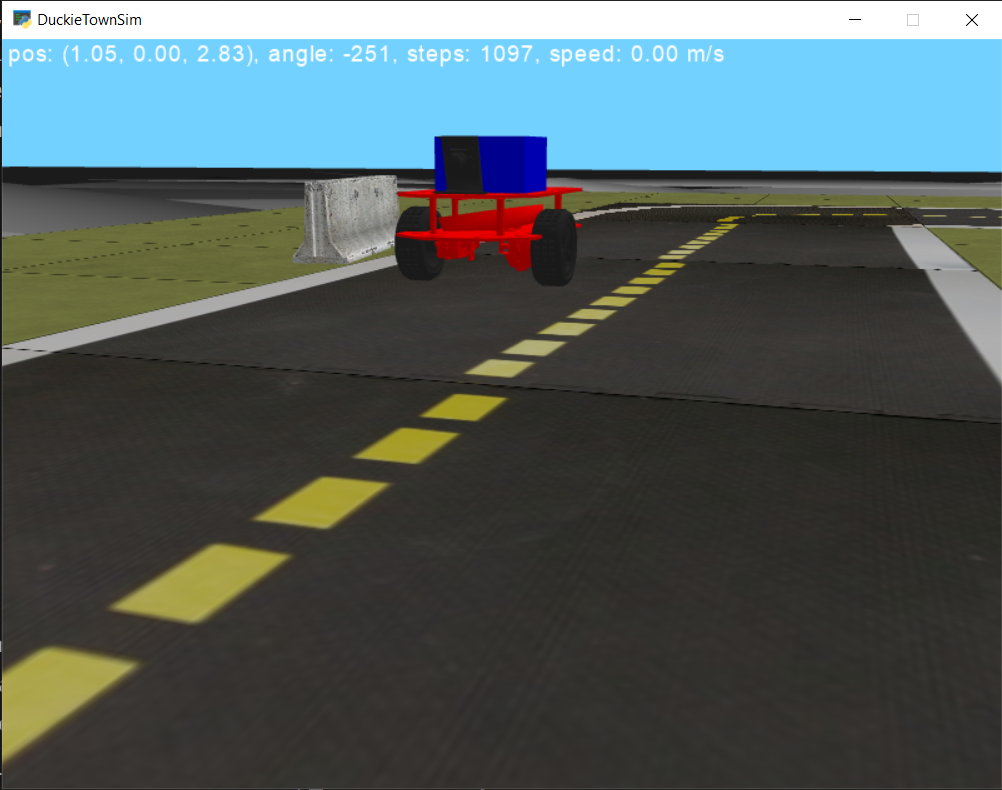
\includegraphics[width=1\linewidth]{4/loop dyn bots.png}
    \caption{Loop\_dyn\_duckiebots Environment}
    \label{fig:loop_dyn_duckiebots}
\end{figure}

\section{DATASET}

In fig \ref{fig:processed_dataset}, we can see the dataset generate by the Dataset Collection Tool. It is stored in .pkl format. The dataset's columns are: i) Video Description, ii) Action to take, iii) Reasoning and iv) predict the next control signals.

Dataset Preparation:
\begin{itemize}
    \item Collect a diverse set of videos relevant to the task at hand.
    \item Annotate the videos with frame-level labels if necessary for supervised learning.
    \item Preprocess the videos to a consistent format and resolution.
    \item Split the dataset into training, validation, and test sets.
\end{itemize}


\begin{figure}
    \centering 
    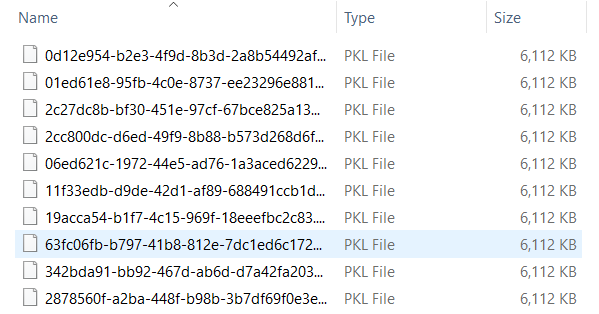
\includegraphics[width=1\linewidth]{4/processed_dataset.png}
    \caption{Dataset}
    \label{fig:processed_dataset}
\end{figure}
\section{VISION ENCODER}
In \ref{algo:encoder}, we can see the algorithm for Vision Encoder. The vision encoder is implemented in pure python using pytorch's submodules such as nn.Module, autograd etc.

The alignment head is implemented using nn.Module and is train on the above collected dataset. The tokenizer and Embedding model is provided by the LLM Module. We are using Swin Transformer for video feature extraction.
\begin{algorithm}
\caption{Video Encoder Architecture}
\begin{algorithmic}
\State \textbf{Input:} Images
\State \textbf{Output:} Video Representation
\State \textbf{Algorithm:}
\State \indent \textbf{Preprocess}
\State \indent \indent Concat the $N$ context sequence images
\State \indent \indent Split the images into smaller $pm1 \times pm2$ image patches
\State \indent \textbf{Linear Projection}
\State \indent \indent Apply Positional Embedding
\State \indent \indent Apply Patch Embedding
\State \indent \indent Concat Positional Embeddings and Patch Embeddings for each Patch
\State \indent \textbf{Vision Transformer} $\to Video Representation$ 

\end{algorithmic}
\label{algo:encoder}
\end{algorithm}

\section{DATA COLLECTION TOOL}
The Data Collection Tool has 2 sub-modules. Their implementations are discussed below

\subsection{Recorder}
In \ref{algo:recorder}, you can see the algorithm of Recorder sub-module in Data Collection Module.
\begin{algorithm}
\caption{Data Recorder Algorithm}
\begin{algorithmic}
\State \textbf{Input:} Screen
\State \textbf{Output:} Clip list
\State \textbf{Algorithm}
\State \indent Focus the window with the title 'Duckietown Sim'
\State \indent Get the window corner coordinates
\State \indent Create a clip list
\State \indent Repeat number of frames per clip times
\State \indent \indent Get screenshot of the window 
\State \indent \indent Add it to the screenshot to the clip list
\State \indent \indent Wait 1//fps secs
\State \indent Return Clip list

\end{algorithmic}
\label{algo:recorder}
\end{algorithm}
\subsection{Data Annotation Tool}  
the data annotation tool is implemented using pysimplegui. A proprietary GUI library in python that is free for use for non-commercial academic purposes. The tool will be replaced by a flask web app for ease of use, accessibility and open-source natures.
\section{CONTROL MODULE}
The Control module is a simple python script which which looks for words such as 'accelerate', 'decelerate', 'turn left' and 'turn right'. Then, converts that words into key presses corresponding to the word given. This is parsed from the model's output parameter 'predicted next control signal'. The current dataset is of the list format which makes it difficult to parse. In future, the format is to be changed to json format.

\end{sloppypar}
 \end{spacing}


% Chapter 5

\chapter{\uppercase{Results and Analysis}} % Main chapter title
\label{chap5} % For referencing
\begin{spacing}{1.5} 
\begin{sloppypar}

Both PHI 2 and PHI 3 can control the ego and seems to maintain the EGO in the road for sometime. 

There is no metric of evaluation established now at this time. 

\section{PHI 2 RESPONSE OUTPUT:}

\shadowbox{
\parbox{300pt}{
\# Action

take soft right and continue straight

\# Reason

Since there the yellow dashed line is slightly towards the right, we take a soft right and continue

\# Next control signal

[('turn right', 'accelerate'),('accelerate',),('accelerate',),
('accelerate',)]}}

\section{PHI 3 RESPONSE OUTPUT:}

\shadowbox{
\parbox{300pt}{
\# Action
\newline
continue straight

\# Reason

Since the road is straight, ego will be centered with the yellow dashed lines without needing to change the direction.

\# Next control Signal

[('accelerate'),('accelerate'),('accelerate'),('accelerate')]
}
}

\section{ANALYSIS}
There is an issue of LLM Module repeating values from a dataset suggests a potential problem in the model's learning process, where it is not generalizing well but rather memorizing and regurgitating information. This could be due to various factors such as overfitting, where the model is too closely aligned with the training data, or a lack of diversity in the dataset, which does not allow the model to learn broader patterns. To address this, further experimentation is indeed crucial. This could involve implementing different model architectures, adjusting hyperparameters, or augmenting the dataset with more varied examples. 

Additionally, the evaluation metrics need to be carefully considered. Traditional metrics like accuracy might not suffice, as they could give a false sense of performance if the model is simply echoing the input data. New metrics that can better capture the model's ability to generalize and provide novel, relevant responses are needed. These could include measures of diversity in the model's outputs, the ability to handle unseen data, or the relevance and usefulness of its responses in practical scenarios. A thorough examination of the model's outputs and a comparison with expected outcomes will be instrumental in diagnosing the underlying issues and guiding the enhancement of the LLM Module's capabilities.

\end{sloppypar}
 \end{spacing}
\include{6/Chapter6}
\chapter{\uppercase{Conclusion and Future Work}}
\label{chap:conclusion}
\begin{spacing}{1.5}
\begin{sloppypar}
\section{\uppercase{CONCLUSION}}
The advent of knowledge-driven autonomous driving agents heralds a transformative era in the realm of transportation, signaling the impending reality of driverless cars. This innovative approach leverages the vast potential of machine learning and artificial intelligence to navigate complex environments with a level of precision and adaptability previously unattainable. The significance of this project lies not only in its forward-thinking vision but also in its feasibility within low-resource settings, demonstrating that cutting-edge research and development in autonomous driving technology are not confined to high-end laboratories with abundant funding. It underscores the accessibility of such technologies, paving the way for widespread adoption and iterative improvement.

Furthermore, the project showcases the versatility of Large Language Models (LLMs) as a core component of autonomous driving systems. LLMs' ability to interpret and process vast amounts of data in real-time allows them to make informed decisions, enhancing the safety and reliability of autonomous vehicles. Their expandability ensures that as the technology evolves and new data becomes available, the driving agents can be updated and improved, thus future-proofing the system. The generalizability of LLMs means they can be adapted to various driving conditions and geographies, making them a robust foundation for global deployment.

This project's implications extend beyond the technical sphere, promising to revolutionize how society views mobility and accessibility. By reducing the reliance on human drivers, it opens up new opportunities for individuals who may be unable to drive due to physical limitations or other constraints. It also has the potential to significantly decrease traffic accidents caused by human error, thereby improving road safety. The environmental impact cannot be overlooked either; autonomous driving agents can optimize routes and driving patterns to reduce fuel consumption and emissions.

In conclusion, the development of knowledge-driven autonomous driving agents is a monumental step towards an autonomous future. It embodies the synergy between theoretical research and practical application, illustrating that even with limited resources, significant strides can be made in this cutting-edge field. As LLMs continue to evolve, their interpretability, expandability, and generalizability will only enhance the capabilities of autonomous driving agents, making the dream of driverless cars an imminent reality. The project not only contributes to the technological landscape but also has far-reaching effects on societal norms, safety, and the environment, marking a pivotal moment in the journey towards sustainable and intelligent transportation systems.
\section{\uppercase{FUTURE WORK}}
The future expansion of this work holds promising avenues for enhancing the robustness and applicability of the research. Firstly, the creation of more dataset data is crucial. This involves not only increasing the volume of data but also ensuring its diversity to cover a wide array of scenarios that the models may encounter. This could include varied environmental conditions, different geographic locations, and a multitude of operational contexts. 

Secondly, comparing newer and bigger models can provide insights into the scalability and efficiency of current algorithms. As computational power increases and new architectures are developed, it is imperative to assess their performance against established benchmarks. This comparison could lead to the discovery of more sophisticated models that offer improved accuracy and speed.

Enabling fine-tuning is another significant step. This process allows models to be more precisely adjusted to specific tasks by training on a smaller, task-specific dataset after being pre-trained on a large dataset. Fine-tuning can result in models that perform better on specialized tasks, adapting to the nuances of the data they are meant to interpret.

Testing in new maps is essential for validating the generalizability of the models. By exposing the models to previously unseen environments, researchers can evaluate their adaptability and identify areas where further training is needed. This helps in ensuring that the models are not just theoretically sound but also practically viable.

Lastly, rewriting the Dataset Collection tool to be a web app can significantly streamline the data collection process. A web-based tool can be more accessible to users, allowing for easier data input and management. It can also facilitate real-time data collection and analysis, which is invaluable for dynamic research environments.

Each of these steps is designed to build upon the existing foundation, pushing the boundaries of what is currently possible and paving the way for new discoveries in the field. The continuous evolution of technology necessitates an iterative approach to research, where each phase of expansion is seen as an opportunity to refine and enhance the work being done. The integration of these expansions will undoubtedly lead to more sophisticated and capable systems, driving progress in the field forward.
 \end{sloppypar}
 \end{spacing}
\cleardoublepage
\phantomsection 
\include{Appendix/appendix}


%\bibliographystyle{auapalike}
\bibliographystyle{unsrt}
\nocite{*}%This gives a list of all references that includes without citation. Remove this, once the reference is cited
\phantomsection
\addcontentsline{toc}{chapter}{REFERENCES}
\begin{spacing}{1}
\bibliography{publication}
\end{spacing}

\newpage
\clearpage




\addtocontents{toc}{\protect\newpage}
\addtocontents{lot}{\protect\newpage}
\addtocontents{lof}{\protect\newpage}

\end{document}
